\documentclass[asi]{picINSA}
\DeclareGraphicsRule{*}{pdf}{*}{}
\usepackage{pdfpages}

%\usepackage{colortbl}
\usepackage{fancyhdr}
\usepackage{listings} 
\usepackage{mathrsfs}
\usepackage{url}
\usepackage{lmodern}
\usepackage{color}
\usepackage{xcolor}
\usepackage{wrapfig}
\usepackage{graphicx}
\usepackage{pdflscape}
\usepackage{longtable}
\usepackage{sectsty}
\usepackage{lastpage}
\usepackage{multirow}
\usepackage{float}
\usepackage{eso-pic}
\usepackage[french]{minitoc}
\usepackage[babel=true]{csquotes}
\usepackage{tikz}
\addto\captionsfrench{\def\tablename{Tableau}}
\usepackage{../../ressources/Unipik/vocabulaire/vocabulaireUnipik}
%\usepackage{../../ressources/Unipik/vocabulaire/vocabulaireEastpic}

\setcounter{secnumdepth}{4}
\setcounter{tocdepth}{4}
\newcommand{\ligneMaj}[3] {
	\rowcolor[gray]{0.55} \textbf{\textit{#1}} & #2  &  #3\\
	\hline
}
\newcommand{\ligneSup}[3] {
	\rowcolor[gray]{0.65} |\textunderscore \textbf{\textit{#1}} & #2  &  #3\\
	\hline
}
\newcommand{\ligneMed}[3] {
	\rowcolor[gray]{0.75} \hspace{0.25cm} |\textunderscore #1  & #2 & #3 \\
	\hline
}
\newcommand{\ligneSub}[3] {
	\rowcolor[gray]{0.85}  \hspace{0.5cm} |\textunderscore #1 & #2 & #3\\
	\hline
}
\newcommand{\ligneSubSub}[3] {
	\rowcolor[gray]{0.95}  \hspace{0.75cm} |\textunderscore #1 & #2 & #3\\
	\hline
}
\newcommand{\ligneTache}[3] {
	\hspace{1.00cm} |\textunderscore #1 & #2 & #3\\
	\hline
}
\title{\PQ{}}
\author{\Pierre}


\titreGeneral{\PQ}
\sousTitreGeneral{\nomEquipe}
\titreAcronyme{\PQCourt}
\version{V1.00}
\titreDetaille{\PQCourt\_Q\_\nomEquipe\_\versionPrive}
\referenceVersion{\PQCourt\_Q\_\nomEquipe\_\versionPrive}
\auteurs{\Kafui{} \& \Melissa{} \& \Sergi{} \& \Michel{} \& \Florian{} \&  \Julie{} \& \Pierre{}}
\destinataires{\nomApprobateur{}, \nomTuteurQualite, \nomEquipe, \nomPIC{}}
\resume{Le présent document contient la présentation du \PQ{} \nomEquipe.}
\motsCles{\PQCourt{}, référentiel, nommage}
\natureDerniereModification{ }
\modeDiffusionControle{}

\begin{document}

\couverture{}

 \informationsGenerales{}
\begin{pagesService}
	\begin{historique}
		% nouvelles versions à rajouter AU-DESSUS en recopiant les lignes suivantes et en les modifiant :
		\unHistorique{1.00}{02/02/2016}{\Sergi \newline \Pierre \newline \Michel}{Création}{Toutes}

	\end{historique}

        \begin{suiviDiffusions}

            % On place ici les diffusions
        	\unSuivi{1.00}{}{\nomEquipe{}, \nomPIC{}}
          
          
        \end{suiviDiffusions}

%%Signataires
        \begin{signatures}
	   \uneSignature{Vérificateur}{\RQ{},\newline \CPA}{\Pierre{}}{26/01/2016}{courriel}
       \uneSignature{Validateur}{\CP{}}{\Sergi}{26/01/2016}{courriel}
	   \uneSignature{Approbateur}{Le client}{\nomClient}{}{}
        \end{signatures}
	
	

	
	
\end{pagesService}


\tableofcontents

\setcounter{chapter}{0}
 
\chapter{Fiche projet}
\label{fiche_projet}
		Le présent document présente le \PQ{} du PIC UNICEF qui sera désigné sous le nom de "\nomEquipe" pour tous les documents liés à ce PIC. L'objectif de ce \PQ{} est de décrire l'ensemble des modes opératoires, des ressources et de la séquence des activités liées à ce projet. Il aide à démontrer que \nomEquipe{} est capable de fournir un produit conforme aux exigences du client et à la norme \ISO . \\
		
		Des contrôles réguliers seront effectués afin de vérifier la bonne application de la démarche décrite dans ce \PQ .\\
		
		La direction ainsi que l'ensemble des membres de l'équipe \nomEquipe{} s'engagent à respecter les dispositions décrites dans ce \PQ .\\ 
		

		
	\begin{description}
		\item[Sujet du PIC~:] "L'objectif est de permettre une gestion informatisée par les divers responsables des actions et des comités départementaux des actions à venir, en cours et passées" sur les trois programmes suivants : plaidoyers, les poupées Frimousse et les actions liées aux Jeunes Ambassadeurs \\	
		\item[Intitulé du PIC~:] PIC \nomPIC \\	
		\item[Nom de l'équipe PIC~:] \nomEquipe \\
	\end{description}


\noindent\hfil\rule{\textwidth}{.4pt}\hfil


		
\section*{Cahier des charges}
		\subsection*{Besoin à satisfaire~:} 
			cf. \DSE . 		
		\subsection*{Element à livrer~:}
			cf. \DSE
			
					


	\vspace{1cm}
	\noindent\hfil\rule{\textwidth}{.4pt}\hfil
	\vspace{1cm}	
	
	
\section*{Information sur le client}
	\begin{description}
		\item[Nom de l'organisme~:] UNICEF Haute Normandie \\
		\item[Nom de son représentant~:] Véronique BARBIER \\
		\item[Adresse de l'organisme~:] 12 rue  du Dr Chanoine, 27200 Vernon \\
		\item[Téléphone~:] 02 32 54 92 50 \\
		\item[E-mail~:] president.unicef76@unicef.fr \\
	\end{description}
	
	
	\vspace{1cm}
	\noindent\hfil\rule{\textwidth}{.4pt}\hfil
	\vspace{1cm}	
	
\section*{Informations complémentaires}
	
	\begin{description}
	
		\item[Nom du tuteur pédagogique~:] \nomTuteurPedago \\
		\item[Nom du tuteur qualité~:] \nomTuteurQualite \\
		\item[Lieu de réalisation du projet~:] \adresseSalle \\
		\item[Nombre d'élève ingénieur de l'équipe PIC~:] 9 \\
	\end{description}	
	
	\noindent\hfil\rule{\textwidth}{.4pt}\hfil	
	
	\section*{Aspect contractuel}
	
	
	\begin{tabular}[h]{|p{0.3\textwidth}|p{0.6\textwidth}|}
	\hline
	
	\cellcolor{gray!40}Membre équipe PIC & \cellcolor{gray!40}Rôle(s) \\\hline
	\Sergi & \CP \\\hline
	\Pierre & \CPA , \RQ \\\hline
	\Michel & \D , \RD \\\hline 
	\Kafui  & \D , \RQA \\\hline
	\Matthieu & \D , \RRS \\\hline
	\Mathieu & \D , \RGC \\\hline
	\Melissa  & \D \\\hline
	\Julie & \D \\\hline
	\Florian & \D \\\hline
	
\end{tabular}
	
	\vspace{1cm}
	\noindent\hfil\rule{\textwidth}{.4pt}\hfil
	\vspace{1cm}	
	
	\section*{Propriété intellectuelle}
		\begin{itemize}
			\item Copropriété $\square$
			\item Propriété INSA $\square$
			\item Propriété entreprise $\boxtimes$
		\end{itemize}
	
		


\chapter{Engagements}
\label{egagements}
Tous les signataires ont pris connaissance du présent Plan Qualité et s'engagent à respecter ses exigences. \\
	
	\vspace{1cm}

\begin{tabular}[h]{|p{0.25\textwidth}|p{0.40\textwidth}|p{0.12\textwidth}|p{0.12\textwidth}|}
	\hline
	
	\cellcolor{gray!40}Membre équipe PIC & \cellcolor{gray!40}Rôle(s) dans le projet & \cellcolor{gray!40}Date & \cellcolor{gray!40}Signature \\\hline
	\Sergi & \CP & 27/01/2016 &  \\\hline
	\Pierre & \RQ \newline \CPA & 27/01/2016 &  \\\hline
	\Michel & \D \newline \RD & 27/01/2016 &  \\\hline
	\Kafui & \D \newline \RQA & 27/01/2016 &  \\\hline
	\Matthieu & \D \newline \RRS & 27/01/2016 &  \\\hline
	\Mathieu & \D \newline \RGC & 27/01/2016 &  \\\hline
	\Melissa & \D & 27/01/2016 &  \\\hline
	\Julie & \D & 27/01/2016 &  \\\hline
	\Florian & \D & 27/01/2016 &  \\\hline
\end{tabular}


\chapter{Décomposition en fonction des membres (WBS)}
\label{decomp_membre_WBS}
\section{Décomposition en activités des processus du PIC}

Le Système de Management de la Qualité défini par le PIC \nomPIC{} se décompose en trois processus~:
\begin{itemize}
 \item Manager la qualité : assurer, suivre et améliorer la qualité udu pic ; 
 \item Conduire le projet ;
 \item Réaliser les produits. \\
\end{itemize}

Un pilote (membre de PIC) est attribué à chaque processus. Sa mission sera de s'assurer du bon fonctionnement du processus et de gérer les risques liés à ce dernier.

Pour diviser le projet en processus, nous avons utilisé un Work Breakdown Structure(WBS). Le WBS est visible sur la figure \ref{WBS1}.

\begin{figure}[H]
\centering
 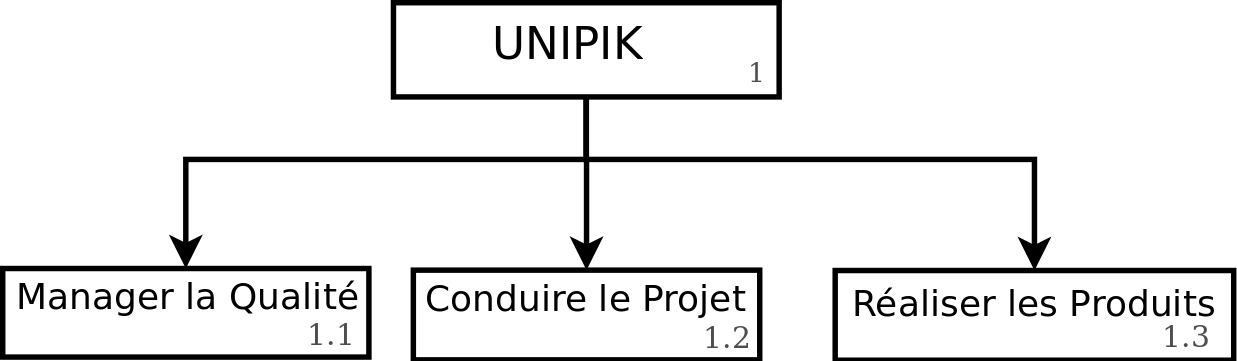
\includegraphics[width=14cm]{images/organigrammeProcessusPic.png}
 \caption{Processus du PIC~: projet \nomEquipe{}}
 \label{WBS1}
\end{figure}

 Dans le cas ou il y a des évolutions, les modifications seront présentées dans la prochaine mise à jour.
\newpage
 
\section{Processus : Manager la Qualité}
\label{ProcessusQualite}
Ce processus se décompose en trois parties~:
\begin{itemize}
\item La mise en place de la Qualité au sein du PIC (rédaction du PQ et organisation de l'équipe PIC) ; 
\item Le suivi de la Qualité tout au long du projet ; 
\item L'amélioration de la Qualité tout au long du PIC (définition d'objectifs et d'axes d'amélioration et mise à jour des documents). 
\end{itemize}
\subsection{\WBSCourt{}}
Le Système de Management de la Qualité au moment de la diffusion de ce document est présenté par une WBS, disponible en figure 3.2.
Le pilote de ce processus sera \Pierre{} en tant que \RQ{}.

\begin{figure}[H]
\centering
 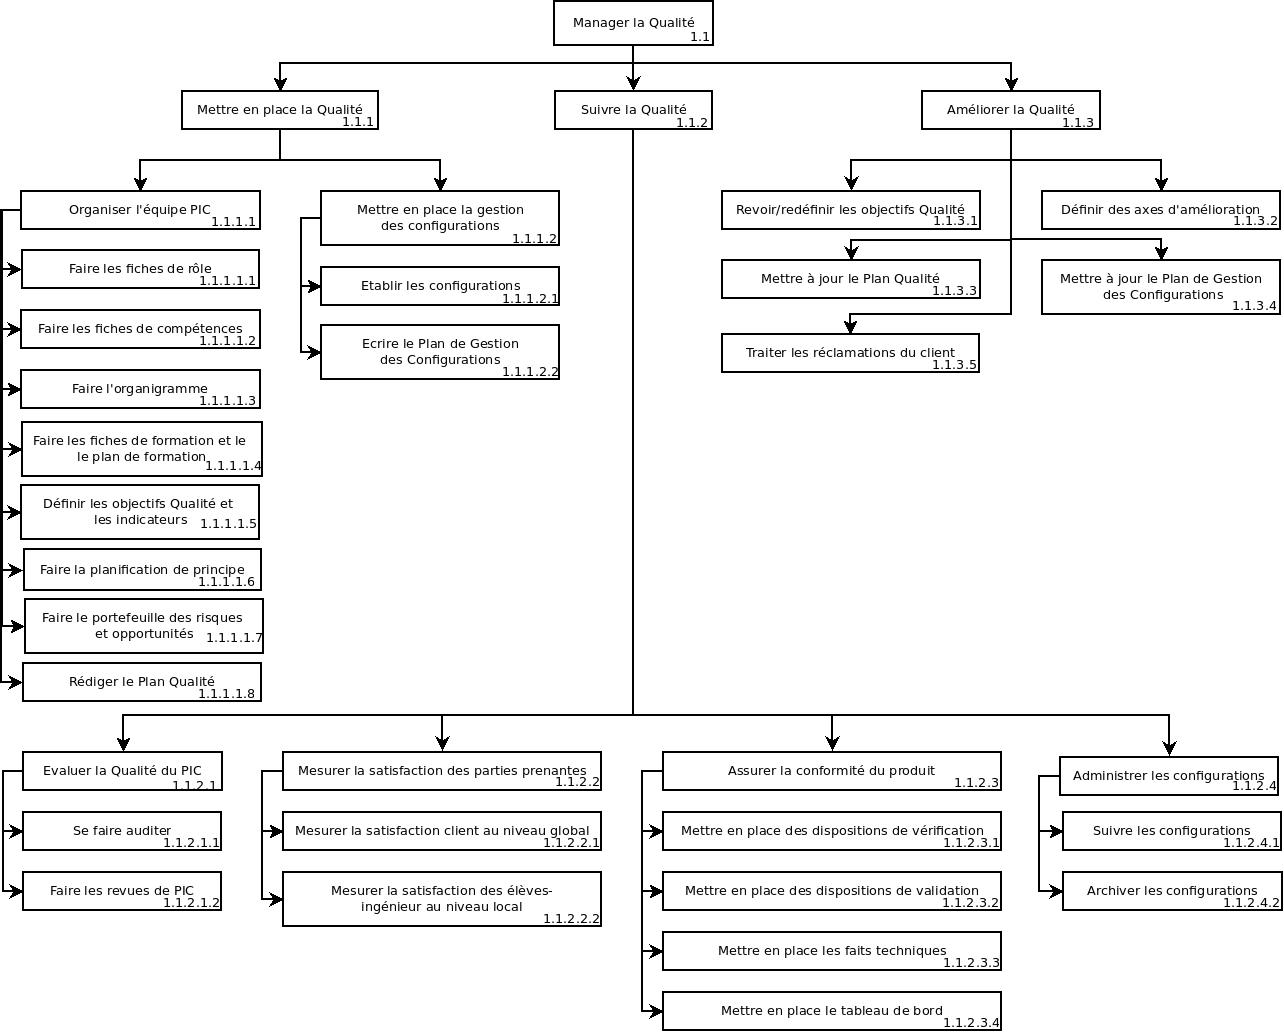
\includegraphics[width=19cm,angle=-90]{images/managerQualite.png}
 \caption{\WBSCourt{}~: Manager la Qualité}
 \label{WBS2}
\end{figure}

\newpage

\subsection{Références aux procédures}
\begin{landscape}
\begin{longtable}{|p{3.0cm}|p{14.5cm}|p{5cm}|}
	% En-tête du tableau
	\hline
	\rowcolor[gray]{0.65}\textbf{N° WBS} & \textbf{Intitulé du processus / de l'activité / de la tâche} & \textbf{Procédure en référence}\\
	\hline
	\endhead % (répétée, sinon \endfirsthead)

	% Corps du tableau


        \ligneMaj{1.1}{Manager la qualité}{Chapitre 4 - \DGQDEUXCourt{}}

        \ligneSup{1.1.1}{Mettre en place la qualité}{Partie 4.2 - \DGQDEUXCourt{}}
        \ligneMed{1.1.1.1}{Organiser l'équipe PIC}{Partie \ref{Organisation} - \PQCourt{}}
        \ligneSub{1.1.1.1.1}{Faire les fiches de rôle}{Partie 3.2.2 - \DGQDEUXCourt{}}
        \ligneSub{1.1.1.1.2}{Faire les fiches de compétences}{Partie \ref{CompetencesEtFormations} - \PQCourt{}}
        \ligneSub{1.1.1.1.3}{Faire l'organigramme}{Partie \ref{CompetencesEtFormations} - \PQCourt{}}
        \ligneSub{1.1.1.1.4}{Faire les fiches de formation et le plan de formation}{Partie \ref{CompetencesEtFormations} - \PQCourt{}}
        \ligneSub{1.1.1.1.5}{Définir les objectifs Qualité et les indicateurs}{Partie \ref{Organisation} - \PQCourt{}}
        \ligneSub{1.1.1.1.6}{Faire la planification de principe}{Partie \ref{CompetencesEtFormations} - \PQCourt{}}
        \ligneSub{1.1.1.1.7}{Faire le portefeuille des risques et opportunités}{Partie \ref{CompetencesEtFormations} - \PQCourt{}}
        \ligneSub{1.1.1.1.8}{Rédiger le Plan Qualité}{Partie 4.2.2 - \DGQDEUXCourt{}}
        \ligneMed{1.1.1.2}{Mettre en place la gestion des configurations}{Partie 7.2 - \DGQDEUXCourt{}}

        \ligneSup{1.1.2}{Suivre la Qualité}{Partie 4.3 - \DGQDEUXCourt{}}
        \ligneMed{1.1.2.1}{Evaluer la Qualité du PIC}{}
        \ligneSub{1.1.2.1.1}{Se faire auditer}{Partie 4.3.4 - \DGQDEUXCourt{}}
        \ligneSub{1.1.2.1.2}{Faire les revues de PIC}{Partie 4.3.3 \DGQDEUXCourt{}}
        \ligneMed{1.1.2.2}{Mesurer la satisfaction des parties prenantes}{Partie 4.3.1 \DGQDEUXCourt{}}
        \ligneSub{1.1.2.2.1}{Mesurer la satisfaction client au niveau global}{Partie 3.1.1 - \DGQTROISCourt{}}
        \ligneSub{1.1.2.2.2}{Mesurer la satisfaction des élèves-ingénieur au niveau local}{Partie 3.1 - \DGQTROISCourt{}}
        \ligneMed{1.1.2.3}{Assurer la conformité du produit}{}
        \ligneSub{1.1.2.3.1}{Mettre en place des dispositions de vérification}{Partie 4.3.2 - \DGQDEUXCourt{}}
        \ligneSub{1.1.2.3.2}{Mettre en place des dispositions de validation}{Partie 4.3.2 - \DGQDEUXCourt{}}
        \ligneSub{1.1.2.3.3}{Mettre en place les faits techniques}{Partie 4.3.5 - \DGQDEUXCourt{}}
        \ligneSub{1.1.2.3.4}{Mettre en place le tableau de bord}{Partie 4.3.6 - \DGQDEUXCourt{}}
        \ligneMed{1.1.2.4}{Administrer les configurations}{Partie 7.3 - \DGQDEUXCourt{}}
        \ligneSub{1.1.2.4.1}{Suivre les configurations}{Partie 8 - \pgcCourt{}}
        \ligneSub{1.1.2.4.2}{Archiver les configurations}{Partie 8 - \pgcCourt{}}

        \ligneSup{1.1.3}{Améliorer la Qualité}{Partie 4.4 - \DGQDEUXCourt{}}
        \ligneMed{1.1.3.1}{Revoir/redéfinir les objectifs Qualité}{Partie 5.2.1 - \DGQTROISCourt{}}
        \ligneMed{1.1.3.2}{Définir des axes d’amélioration}{Partie 4.4.2 - \DGQDEUXCourt{}}
        \ligneMed{1.1.3.3}{Mettre à jour le Plan Qualité}{Partie 4.4.3 - \DGQDEUXCourt{}}
        \ligneMed{1.1.3.4}{Mettre à jour le Plan de Gestion des Configurations}{Partie 4.4.3 - \DGQDEUXCourt{}}
\end{longtable}
\end{landscape}

\newpage



\section{Processus : Conduire le PIC}
\subsection{\WBSCourt{}}
\label{ProcessusConduirePic}
Une WBS qui explique la Conduction du Projet au moment de la diffusion de ce document est disponible en figure 3.3.
Le pilote de ce processus sera \Sergi{} en tant que \CP{}.

\begin{figure}[H]
\centering
 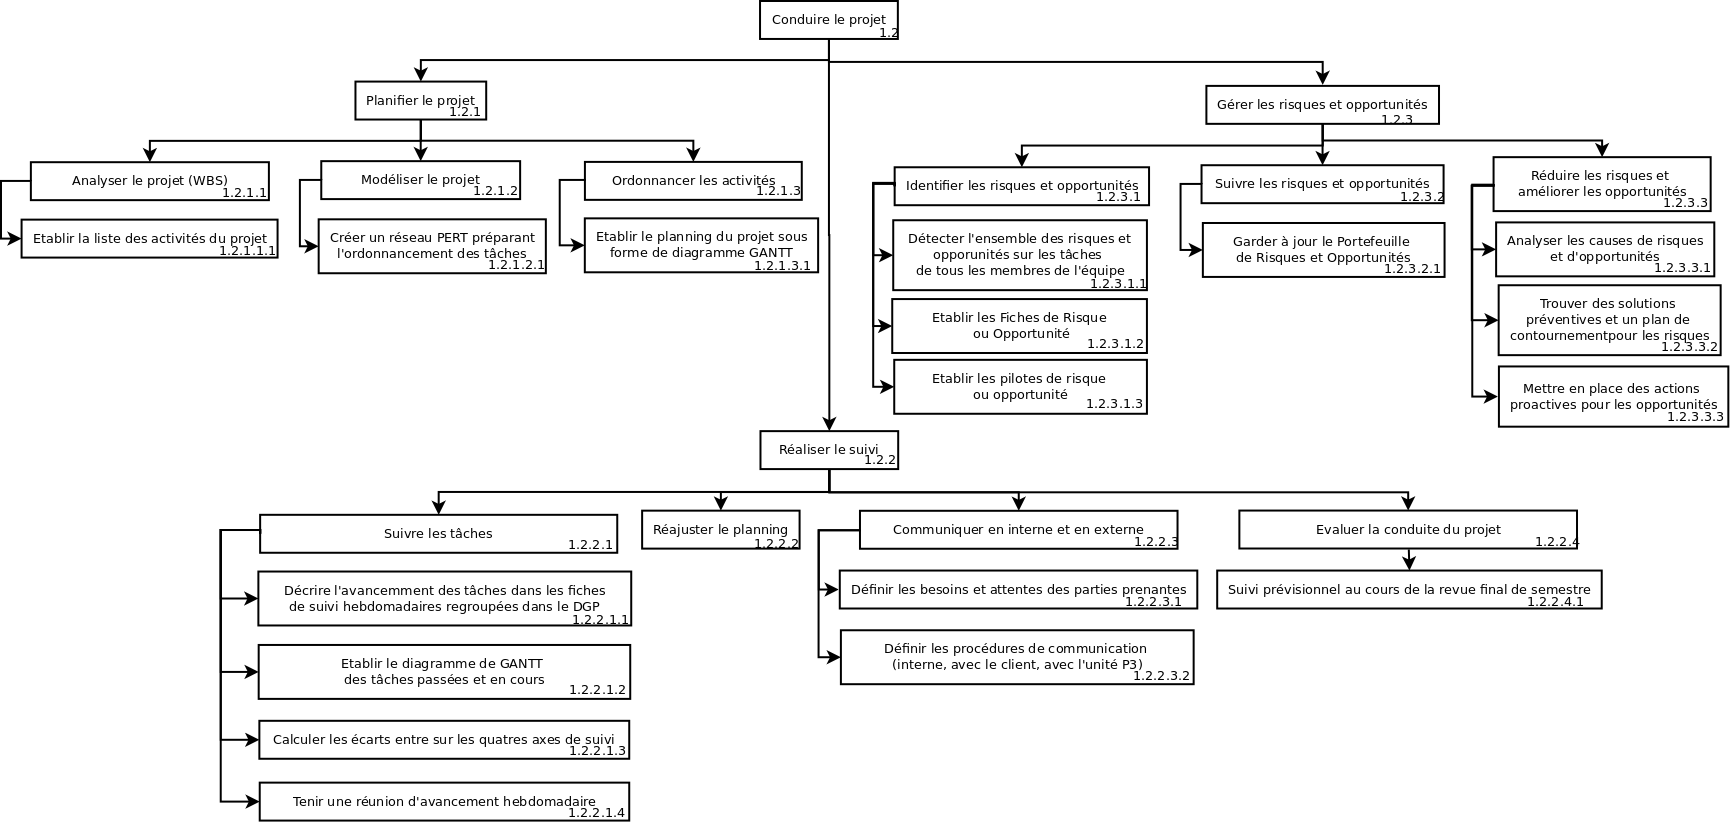
\includegraphics[width=24cm,angle=-90]{images/ConduireLeProjet.pdf}
 \caption{\WBSCourt{}~: Conduire le PIC}
 \label{WBS3}
\end{figure}


\newpage
\begin{landscape}
\subsection{Références aux procédures}
		\small
		\begin{longtable}{|p{3.0cm}|p{14.5cm}|p{5cm}|}
			% En-tête du tableau
			\hline
			\rowcolor[gray]{0.65}\textbf{N° WBS} & \textbf{Intitulé du processus / de l'activité / de la tâche} & \textbf{Procédure en référence}\\
			\hline
			\endhead % (répétée, sinon \endfirsthead)

			\ligneMaj{1.2}{Conduire le projet}{Chapitre 5 - \DGQDEUXCourt{}}

			\ligneSup{1.2.1}{Planifier le projet}{Partie 5.2 - \DGQDEUXCourt{}}
			\ligneMed{1.2.1.1}{Analyser le projet (WBS)}{Partie 5.2.1 - \DGQDEUXCourt{}}
			\ligneSub{1.2.1.1.1}{Établir la liste des activités du projet}{}
			\ligneMed{1.2.1.2}{Modéliser le projet}{Partie 5.2.2 - \DGQDEUXCourt{}}
			\ligneSub{1.2.1.2.1}{Créer un réseau PERT préparant l'ordonnancement des tâches}{}
			\ligneMed{1.2.1.3}{Ordonnancer les activités}{Partie 5.2.3 - \DGQDEUXCourt{}}
			\ligneSub{1.2.1.3.1}{Établir le planning du projet sous forme de diagramme GANTT}{}


			\ligneSup{1.2.2}{Réaliser le suivi}{Partie 5.3 - \DGQDEUXCourt{}}
			\ligneMed{1.2.2.1}{Suivre les tâches}{Partie 5.3.1 - \DGQDEUXCourt{}}
			\ligneSub{1.2.2.1.1}{Décrire l’avancement de ses tâches dans les fiches de suivi hebdomadaires regroupées dans le DGP}{}
			\ligneSub{1.2.2.1.2}{Établir le diagramme de GANTT des tâches passées et en cours}{}
			\ligneSub{1.2.2.1.3}{Calculer les écarts entre sur les quatre axes de suivi}{}
			\ligneSub{1.2.2.1.4}{Tenir une réunion d'avancement hebdomadaire}{}
			\ligneMed{1.2.2.2}{Réajuster le planning}{Partie 5.3.2 - \DGQDEUXCourt{}}
			\ligneMed{1.2.2.3}{Communiquer en interne et en externe}{Partie 5.3.3 - \DGQDEUXCourt{}}
			\ligneSub{1.2.2.3.1}{Définir les besoins et attentes des parties prenantes}{}
			\ligneSub{1.2.2.3.2}{Définir les procédures de communication (interne, avec le client, avec l'unité P3)}{}
			\ligneMed{1.2.2.4}{Évaluer la conduite du projet}{Partie 5.3.4 - \DGQDEUXCourt{}}
			\ligneSub{1.2.2.4.1}{Suivi prévisionnel au cours de la revue final de semestre}{}

			\ligneSup{1.2.3}{Gérer les risques et opportunités}{Partie 5.4 - \DGQDEUXCourt{}}
			\ligneMed{1.2.3.1}{Identifier les risques et opportunités }{Partie 5.4.1 - \DGQDEUXCourt{}}
			\ligneSub{1.2.3.1.1}{Détecter l'ensemble des risques sur les tâches de tous les membres de l'équipe}{}
			\ligneSub{1.2.3.1.2}{Établir les Fiches de Risque ou Opportunité}{}
			\ligneSub{1.2.3.1.3}{Établir les pilotes de risque ou opportunité}{}
			\ligneMed{1.2.3.2}{Suivre les risques et opportunités}{Partie 5.4.2 - \DGQDEUXCourt{}}
			\ligneSub{1.2.3.2.1}{Garder à jour le Portefeuille de Risques et Opportunités}{}
			\ligneMed{1.2.3.3}{Réduire les risques et améliorer les opportunités}{Partie 5.4.3 - \DGQDEUXCourt{}}
			\ligneSub{1.2.3.3.1}{Analyser les causes de risques et d'opportunités}{}
			\ligneSub{1.2.3.3.2}{Trouver des solutions préventives et un plan de contournement pour les risques}{}
			\ligneSub{1.2.3.3.3}{Mettre en place des actions proactives pour les opportunités}{}
		\end{longtable}
	\end{landscape}

	\normalsize
	\newpage

\section{Processus : Réaliser les produits}
\subsection{\WBSCourt{}}
\label{ProcessusRealiserProduit}
Une WBS représentant la réalisation des produits au moment de la diffusion du présent document est disponible en figure \ref{WBS5}.
Le pilote de ce processus sera \Michel{} en tant que \RD{}.

\begin{figure}[H]
\centering
 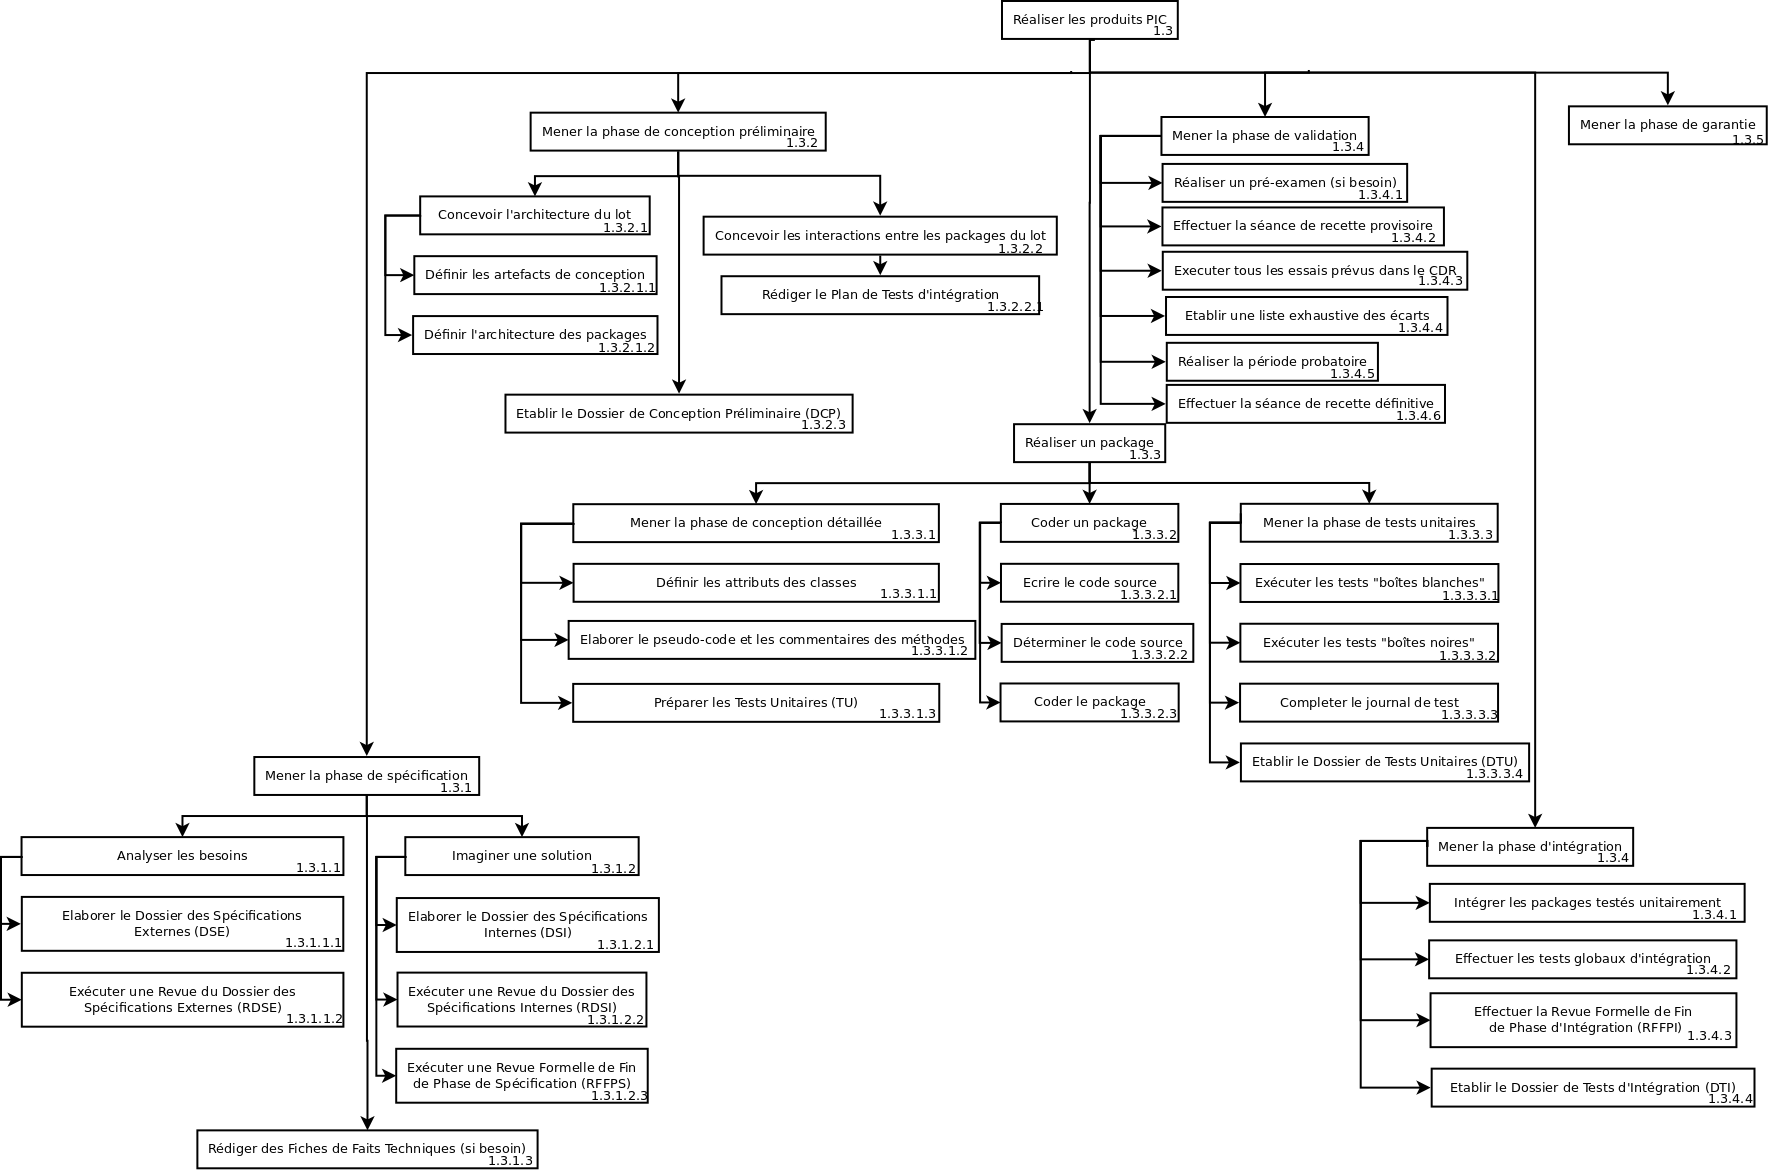
\includegraphics[width=24cm,angle=-90]{images/RealiserProduits.pdf}
 \caption{\WBSCourt{}~: Réaliser les produits}
\label{WBS5}
\end{figure}


\newpage
\begin{landscape}
\subsection{Références aux procédures}
		\begin{longtable}{|p{3.0cm}|p{14.5cm}|p{5cm}|}
		% En-tête du tableau
		\hline
		\rowcolor[gray]{0.65}\textbf{N° WBS} & \textbf{Intitulé du processus / de l'activité / de la tâche} & \textbf{Procédure en référence}\\
		\hline
		\endhead % (répétée, sinon \endfirsthead)

		\ligneMaj{1.3}{Réaliser les produits}{Chapitre 6 - \DGQDEUXCourt{}}

		\ligneSup{1.3.1}{Mener la phase de spécification}{Partie 6.2 - \DGQDEUXCourt{}}
		\ligneMed{1.3.1.1}{Analyser les besoins}{}
		\ligneSub{1.3.1.1.1}{Elaborer le Dossier des Spécifications Externes (DSE)}{Partie 6.2.1 - \DGQDEUXCourt{}}
		\ligneSub{1.3.1.1.2}{Exécuter une Revue du Dossier des Spécifications Externes (RDSE)}{Partie 6.2.2 - \DGQDEUXCourt{}}
		\ligneMed{1.3.1.2}{Imaginer une solution}{}
		\ligneSub{1.3.1.2.1}{Elaborer le Dossier des Spécifications Internes (DSI)}{Partie 6.2.1 - \DGQDEUXCourt{}}
		\ligneSub{1.3.1.2.2}{Exécuter une Revue du Dossier des Spécifications Internes (RDSI)}{Partie 6.2.2 - \DGQDEUXCourt{}}
		\ligneSub{1.3.1.2.3}{Exécuter une Revue Formelle de Fin de Phase de Spécification (RFFPS)}{Partie 6.2.4 - \DGQDEUXCourt{}}
		\ligneMed{1.3.1.3}{Rédiger des Fiches de Faits Techniques (si besoin)}{Partie 6.2.3 - \DGQDEUXCourt{}}

		\ligneSup{1.3.2}{Mener la phase de conception préliminaire}{Partie 6.3 - \DGQDEUXCourt{}}
		\ligneMed{1.3.2.1}{Concevoir l'architecture du lot}{}
		\ligneSub{1.3.2.1.1}{Définir les artefacts de conception}{Partie 6.3.1 - \DGQDEUXCourt{}}
		\ligneSub{1.3.2.1.2}{Définir l'architecture des packages}{Partie 6.3.3 - \DGQDEUXCourt{}}
		\ligneMed{1.3.2.2}{Concevoir les interactions entre les packages du lot}{}
		\ligneSub{1.3.2.2.1}{Rédiger le Plan de Tests d'intégration}{Partie 6.3.5 - \DGQDEUXCourt{}}
		\ligneSub{1.3.2.3}{Établir le Dossier de Conception Préliminaire (DCP)}{Partie 6.3.4 - \DGQDEUXCourt{}}

		\ligneSup{1.3.3}{Réaliser un package}{Partie 6.4 - \DGQDEUXCourt{}}
		\ligneMed{1.3.3.1}{Mener la phase de conception détaillée}{Partie 6.4.1 - \DGQDEUXCourt{}}
		\ligneSub{1.3.3.1.1}{Définir les attributs des classes}{Partie 6.4.1 - \DGQDEUXCourt{}}
		\ligneSub{1.3.3.1.2}{Élaborer le pseudo-code et les commentaires des méthodes}{Partie 6.4.1 - \DGQDEUXCourt{}}
		\ligneSub{1.3.3.3.3}{Préparer les Tests Unitaires (TU)}{Partie 6.4.1 - \DGQDEUXCourt{}}
		\ligneMed{1.3.3.2}{Coder un package}{Partie 6.4.2 - \DGQDEUXCourt{}}
		\ligneSub{1.3.3.2.1}{Écrire le code source}{Partie 6.4.2 - \DGQDEUXCourt{}}
		\ligneSub{1.3.3.2.2}{Déterminer le code source}{Partie 6.4.2 - \DGQDEUXCourt{}}
		\ligneSub{1.3.3.2.3}{Coder le package}{Partie 6.4.2 - \DGQDEUXCourt{}}
		\ligneMed{1.3.3.3}{Mener la phase de tests unitaires}{Partie 6.4.3 - \DGQDEUXCourt{}}
		\ligneSub{1.3.3.3.1}{Exécuter les tests "boîtes blanches"}{Partie 6.4.3 - \DGQDEUXCourt{}}
		\ligneSub{1.3.3.3.2}{Exécuter les tests "boîtes noires"}{Partie 6.4.3 - \DGQDEUXCourt{}}
		\ligneSub{1.3.3.3.3}{Compléter le journal de test}{Partie 6.4.3 - \DGQDEUXCourt{}}
		\ligneSub{1.3.3.3.4}{Établir le Dossier de Tests Unitaires (DTU)}{Partie 6.4.3 - \DGQDEUXCourt{}}

		\ligneSup{1.3.4}{Mener la phase d'intégration}{Partie 6.5 - \DGQDEUXCourt{}}
		\ligneMed{1.3.4.1}{Intégrer les packages testés unitairement}{Partie 6.5 - \DGQDEUXCourt{}}
		\ligneMed{1.3.4.2}{Effectuer les tests globaux d'intégration}{Partie 6.5 - \DGQDEUXCourt{}}
		\ligneMed{1.3.4.3}{Effectuer la Revue Formelle de Fin de Phase d’Intégration (RFFPI)}{Partie 6.5 - \DGQDEUXCourt{}}
		\ligneMed{1.3.4.4}{Établir le Dossier de Tests d’Intégration (DTI)}{Partie 6.5 - \DGQDEUXCourt{}}

		\ligneSup{1.3.4}{Mener la phase de validation}{Partie 6.6 - \DGQDEUXCourt{}}
		\ligneMed{1.3.4.1}{Réaliser un pré-examen}{Partie 6.6.1 - \DGQDEUXCourt{}}
		\ligneMed{1.3.4.2}{Réaliser la période probatoire}{Partie 6.6.1 - \DGQDEUXCourt{}}
		\ligneMed{1.3.4.3}{Effectuer la séance de recette provisoire}{Partie 6.6.1 - \DGQDEUXCourt{}}
		\ligneMed{1.3.4.4}{Exécuter tous les essais prévus dans le CDR}{Partie 6.6.1 - \DGQDEUXCourt{}}
		\ligneMed{1.3.4.5}{Établir une lise exhaustive des écarts}{Partie 6.6.1 - \DGQDEUXCourt{}}
		\ligneMed{1.3.4.6}{Effectuer la séance de recette définitive}{Partie 6.6.1 - \DGQDEUXCourt{}}

		\ligneSup{1.3.5}{Mener la phase de garantie}{Partie 6.7 - \DGQDEUXCourt{}}
		\end{longtable}
\end{landscape}

\chapter{Procédures et description de la gestion de projet}
\label{gestion_projet}
Le processus de \textit{gestion de projet} se décompose en trois sous processus : 
\begin{itemize}
\item Planifier le projet
\item Réaliser le suivi
\item Gérer les risques et opportunités
\end{itemize}

\section{Planification du projet}
\label{planification}

Le processus \textit{Planifier le projet} peut se découper en trois sous-processus.

\begin{itemize}
\item Analyser le projet : consiste à établir la liste de l'ensemble des activités du projet.
\item Modéliser le projet : consiste en la création des tâches.
\item Ordonnancer les activités : a pour objectif d'établir un planning du projet, sous la forme d'un diagramme GANTT.
\end{itemize}

Nous étudierons tout d'abord ces trois sous-processus, puis nous présenterons le planning de principe et enfin nous verrons les outils à disposition pour la gestion de projet. 

\subsection{Analyse du projet}
\label{analyse}
Le but de l'analyse est de préparer et de faciliter la modélisation. Nous utiliserons pour cela la structure WBS qui permet de décomposer chaque activité en allant du plus général au particulier. Chaque feuille de la WBS représente une activité. Les WBS proviennent du besoin du client exprimé dans le Cahier des charges et au début de chaque sprint. \\

Dans le cadre de la planification, nous pourrons également utiliser d’autres structures hiérarchiques comme la \FBSCourt (\FBS), l’ OBS (Object \BS) ou encore la \RBSCourt (\RBS). L’analyse du projet va nous permettre de bien préparer l’étape suivante, c’est-à-dire la modélisation.


\subsection{Modélisation du projet}
\label{modelisation}

Au cours de cette modélisation, nous allons reprendre le WBS réalisé lors de l’analyse du projet et nous allons décomposer chaque activité en une ou plusieurs tâches de manière à établir une liste des différentes tâches. Ensuite nous allons définir chaque tâche en précisant sa durée, sa charge, les effectifs en ressources nécessaires et les prédécesseurs de cette tâche. Cette étape va nous aider à préparer l’ordonnancement des tâches.\\

Chaque attribution de tâche se fera via PGPic et/ou sur le kanbanboard utilisé par les membres de l'équipe, notamment pour les tâches de réalisation d’un Sprint. Les tâches seront attribuées aux différents membres de l’équipe PIC en prenant en compte des compétences et des disponibilités de chacun.

\subsection{Ordonnancement}
\label{ordonnancement}

L'objectif de cette phase est d'ordonnancer les activités afin d'établir un planning du projet. Ce planning sera sous la forme d'un GANTT. Ce type de diagramme permet d’avoir une représentation visuelle dans le temps.\\

Pour répertorier les compétences de chacun, des fiches de compétences seront créées au début du projet et mises à jour au fur et à mesure des formations. L’ensemble des formations ainsi que les analyses effectuées sont renseignées dans la Fiche de Suivi des Formations.\\ 

Ce planning sera mis à jour par le \CP{}  ou par son adjoint chaque semaine lors de la réunion d’avancement hebdomadaire. Il sera par la suite disponible sur PGPic.


\subsection{Planning de principe}
\label{planning_de_principe}

Comme dit ci-dessus, le planning du \PICCourt est fait par le \CP{}  et le \CPA{}. Le \RD{}  pourra aussi être sollicité selon le type de tâche.

\subsection*{Semestre 1 : Janvier 2016 - Mai 2016}

Durant le premier semestre, nous disposons de 12 semaines de \PICCourt. Le planning global sera donc le suivant : 
\begin{itemize}
\item Installation, initialisation des procédures de qualité, prise en main des technologies internes (1 semaine);
\item Premier sprint: réalisation du 1er lot (4 semaines);
\item Deuxième sprint (4 semaines);
\item Troisième sprint: finalisation du 2ème lot (3 semaines);
\end{itemize}

\subsection*{Semestre 2 : Septembre 2016 - Janvier 2017}

Durant le second semestre, nous disposons de 14 semaines de \PICCourt. Le planning global sera donc le suivant : 
\begin{itemize}
\item Quatrième sprint: réalisation du 3ème lot (6 semaines);
\item Cinquième sprint (4 semaines);
\item Sixième sprint: finalisation du 4ème lot (4 semaines);\\
\end{itemize}

Ce planning est théorique et pourra être modifié à l'avenir. 

\subsection{Outils pour la gestion du projet}
\label{outils_gestion}

Nous allons présenter dans cette partie le logiciel et les méthodes utilisés pour la gestion du \PICCourt. \\

\subsubsection*{PGPic}

PGPic est un logiciel développé initialement par l'équipe Geotopic, une équipe \PICCourt de l'\INSACourt. Il est utilisé pour une grande partie de la gestion de projet. \\

Il est disponible à l’adresse \url{https://pgpic.insa-rouen.fr}. Il possède de nombreuses fonctionnalités : 
\begin{itemize}
\item \textbf{Créer et attribuer les tâches}. Le \CP{} définit les tâches pour chaque membre du \PICCourt, et ceux-ci sélectionnent la tâche sur laquelle ils sont en train de travailler. Le \CP{} peut donc voir le temps passé par les membres de son équipe sur chaque tâche, étant donné que PGPic a également un outil de comptage du temps de travail installé sur les machines de la salle \PICCourt ,
\item \textbf{Organiser les tâches}. Le \CP{} peut agencer les tâches en visualisant un diagramme GANTT. Il est possible de retrouver facilement le diagramme GANTT d'une journée particulière car celui-ci est sauvegardé tous les jours, 
\item \textbf{Gérer le suivi des tâches}. Chaque membre peut consulter la fiche de tâche qui le concerne. Ces fiches évoluent chaque jour et sont enregistrées,
\item \textbf{Voir le temps de travail} sur la semaine de chaque membre du \PICCourt. Tous les membres doivent se connecter en arrivant en salle \PICCourt à PGPic, et rester connectés tout au long de leur travail. En fin de semaine, le \CP{} peut donc vérifier si chaque membre du PIC a bien réalisé le nombre d’heures requis,
\item \textbf{Voir le calendrier}. Le Chef PIC peut y ajouter les dates des réunions, audits, fins de sprint, livraisons afin que chaque membre du PIC ait une vision globale des dates limites du semestre. \\ 
\end{itemize}

En revanche, les réclamations du client doivent être prises en compte et PGPic ne permet pas ce suivi. Un autre outil de gestion devra donc être utilisé en parallèle. 


\subsubsection*{Kanbanboards} 

Les Kanbanboards sont des tableaux de suivi des tâches. Celles-ci sont triées dans quatre catégories :
\begin{itemize}
\item \`A faire
\item En cours
\item \`A vérifier
\item Terminé \\ 
\end{itemize}

Nous utiliserons cet outil pour superviser l'avancement technique du projet.

\section{Suivi du projet} 
\label{suivi_projet}

Dans cette partie, nous allons aborder le processus de \textit{Suivi du projet} en étudiant tout d'abord le suivi d'avancement du projet et enfin les communications internes et externes.  

\subsection{Suivi d'avancement}
\label{suivi_avancement}

Nous mettons en place un suivi hebdomadaire ayant pour objectif de mesurer l'avancement du \PICCourt. Nous organiserons entre autre des réunions hebdomadaires qui permettront d'établir et de discuter du planning à venir. Lors de ces réunions, le but est de déclarer et analyser les risques potentiels. Avant chacune de ces réunions, chaque membre du PIC doit décrire l'avancement des tâches qui lui sont attribuées.\\

À la suite de ces réunions, le \CP{} distribue des éventuelles fiches de tâches modifiées et établit un diagramme de GANTT des tâches futures pour l'ensemble de l'équipe. Un compte rendu sera rédigé à chaque réunion et mis à disposition de l'équipe. \\

De plus, des \textit{daily Scrum} sont mis en place les jours où nous sommes tous présents afin de coordonner les tâches en cours. Le suivi des tâches globales sera fait à l’aide de PGPic.

\subsection{Communication}
\label{communication}

La communication est l'un des aspects les plus importants de la conduite de projet. Nous verrons tout d'abord comment nous communiquons avec les Tuteurs (\tuteurPedagogique{} et \tuteurQualite), ensuite comment s'organise la communication avec le client et enfin les communications internes et inter-\PICCourt.\\ 

Toutes les réunions ne se déroulent pas de la même façon. Cependant, l’archivage d’un compte-rendu se fait toujours en version numérique et parfois en version papier (lorsqu’il est signé).

\subsubsection*{La communication avec les Tuteurs}
La communication se base sur des réunions hebdomadaires par tuteur dont le jour est défini en début de \PICCourt et en cas de besoin, l’envoi de courriels. Des réunions en dehors de ce créneau pourront être organisées exceptionnellement. Ces dernières se déroulent de la façon suivante :
\begin{enumerate}
\item Le \CP{} définit avant chaque réunion un ordre du jour qui recense toutes les questions et points à aborder pendant la réunion. Chaque membre du \PICCourt{} a la possibilité de consulter et de rajouter des éléments à cet ordre du jour. Cela peut se faire par oral ou bien via le bloc-notes de PGPic. 
\item Un secrétaire est désigné à chaque début de réunion pour prendre des notes sur les points abordés et rédiger le compte-rendu au plus tard dans les 7 jours qui suivent.
\item Une fois rédigé, le compte-rendu est soumis à vérification puis validation. Le compte-rendu doit être validé avant la prochaine réunion au plus tard.
\item Une fois validé, le compte-rendu est envoyé au tuteur. Si le compte-rendu n’est pas approuvé, les modifications nécessaires sont apportées, puis il est renvoyé pour approbation.
\item Si le compte-rendu n’est pas approuvé, il est réédité, vérifié, validé et soumis à approbation à la prochaine réunion.
\item Une fois approuvé, le compte-rendu est archivé. 
\end{enumerate}

\subsubsection*{La communication avec le client}

La communication avec le client repose sur : 
\begin{itemize}
\item Des courriels,
\item Des appels,
\item Des réunions entre l'équipe et le client. \\
\end{itemize}

Le \CP{} est l’interlocuteur privilégié du client. En cas d’absence et de nécessité, le \CPA{} peut devenir cet interlocuteur. La fréquence des échanges sera au minimum hebdomadaire. En cas de nécessité, une prise de contact téléphonique peut être initiée par
le client ou le \CP. L’échange d’e-mails est mené depuis l’adresse mise en place dans le cadre des \PICCourt, associée au \CP. Ces e-mails sont archivés et classés selon les libellés définis dans le \PGC. Les réunions avec le client sont prédéfinies à l’avance entre l’équipe \PICCourt et ce dernier. La réunion avec le client se déroule de la façon suivante :
\begin{enumerate}
\item Le \CP{} et le \CPA{} définissent avant chaque réunion un ordre du jour qui recense toutes les questions et points à aborder pendant la réunion. Chaque membre du \PICCourt a la possibilité de consulter et de rajouter des éléments à cet ordre du jour. Cela peut se faire par oral ou bien via le bloc-notes de PGPic.
\item Un secrétaire est désigné à chaque début de réunion pour prendre des notes sur les points abordés et rédiger le compte-rendu au plus tard dans les 7 jours qui suivent.
\item Une fois rédigé, le compte-rendu est envoyé pour vérification puis validation. La validation est obligatoirement effectuée par le \CP.
\item Une fois validé, le compte-rendu est envoyé par courriel au client pour approbation. Si le client ne fait aucune remarque sur le compte-rendu dans les 7 jours suivants l’envoi du mail, le compte-rendu est considéré comme approuvé.
\item Une fois approuvé, le compte-rendu est archivé.
\end{enumerate}


\subsubsection*{Les communications internes}

La communication interne comprend :
\begin{itemize}
\item Des réunions hebdomadaires,
\item Des \textit{Daily Scrum},
\item Des courriels,
\item Groupe Facebook privé. \\
\end{itemize}

Les réunions hebdomadaires auront lieu avec l’équipe au complet. Cette réunion aura pour but de traiter de l’avancement du projet ainsi que de la gestion des risques. Lors de cette réunion seront aussi inspectés les indicateurs de Qualité si ceux-ci sont disponibles au moment de la réunion. De plus, c’est lors de cette réunion que se fera l’attribution des tâches pour la semaine suivante. Avant chaque réunion, un secrétaire est désigné afin de prendre des notes et de rédiger par la suite un compte-rendu qui sera archivé sous forme numérique.\\

Les \textit{Daily Scrum} sont des petites réunions quotidiennes, d’une durée de 15 minutes maximum, s’effectuant debout, le matin. Lors de ces réunions, chaque membre de l’équipe prendra la parole à tour de rôle pour répondre aux questions suivantes :
\begin{itemize}
\item Qu’as-tu fait hier ?
\item Quelles difficultés as-tu rencontré ? Et inversement, de quoi es-tu fier ?
\item Que vas-tu faire aujourd’hui ?
\end{itemize}
Cette réunion permet d’avoir un suivi précis de l’avancement du projet, de soulever d'éventuels problèmes, et d’aider chaque membres à prendre du recul sur les tâches qu’il effectue.\\

Les courriels et le groupe Facebook sont utilisés pour une communication moins formelle. 

\subsubsection*{Les communications inter\picCourt{}}  

Il est important que les équipes des différents \PICCourt puissent communiquer entre elles afin d’échanger des informations concernant le déroulement des \PICCourt et de partager leurs expériences. C'est pourquoi il est important d'organiser des réunions.\\

Les réunions inter\PICCourt{} vont être effectuées soit entre les différents chefs \PICCourt{}, soit entre les différents Responsables Qualité. Le but de ces réunions est de définir des lignes directrices communes aux projets, répondre aux différentes questions qui peuvent survenir lors de la mise en place et du
suivi de la Qualité dans les \PICCourt et prendre des décisions. Elles permettent également d’assurer la Qualité de manière uniforme dans tous les \PICCourt, et de constater les éventuelles différences de Management de la Qualité. Ces réunions donneront lieu à des comptes rendus ou des relevés de décision écrits.

\section{Gestion des risques et opportunités} 
\label{gestion_risques_opportunitees}

Le processus \textit{Gérer les risques et opportunités} est découpé en trois sous-parties : 
\begin{itemize}
\item identifier les risques et opportunités,
\item suivre les risques et opportunités,
\item réduire les risques et améliorer les opportunités. \\
\end{itemize}

L'objectif de la gestion des risques et opportunités est de souligner les points du projet sur lesquels il faut porter une attention particulière. 

\subsection{Identification des risques et opportunités}
\label{identification_risques_opportunitees}

Tous les membres de l'équipe participent à l'identification des risques ou opportunités. Les risques sont identifiés en début de semestre et aboutissent à un \PR. Un portefeuille d'opportunités est également associé aux opportunités identifiées. Cette identification se poursuit tout au long du semestre. Un pilote doit être associé à chaque risque ou opportunité.\\ 

Les risques ou opportunités peuvent être liés :
\begin{itemize}
\item au planning,
\item aux compétences,
\item aux capacités techniques,
\item aux données ou au matériel. \\
\end{itemize}

Les risques ou opportunités peuvent être de différentes natures :
\begin{itemize}
 \item juridique (lié au contrat) ,
 \item technique ,
 \item projet (équipe, organisationnel) ,
 \item externe (conjoncturel) ,
 \item infrastructure (matériel et locaux à disposition de l’équipe \PICCourt) ,
 \item humain. \\
\end{itemize}


\subsubsection*{Les risques}

L'identification des risques a un double objectif : 
\begin{itemize}
\item prévenir l'apparition d'écart par rapport à un objectif ,
\item prévenir l'apparition d'une non-conformité. \\
\end{itemize}
Si un risque est découvert et validé par l'équipe \PICCourt{}, une Fiche de Risques sera rédigée et ajoutée au \PR.\\

Tous les risques n'ont pas le même impact. Celui-ci peut-être :
\begin{itemize}
\item mineur : le risque peut entraîner une difficulté à achever une tâche mais n'entraîne pas de retard ,
\item moyen : le risque peut entraîner un retard sur le projet ,
\item important : le risque entraîne forcement un retard sur le projet ,
\item maximum : le risque bloque le projet.\\
\end{itemize}

La probabilité d'apparition est définie parmi :
\begin{itemize}
 \item peu probable : (P < 20\%) ;
 \item possible : (20\% < P < 40\%) ;
 \item probable : (40\% < P < 60\%) ;
 \item très probable (P > 60\%).\\
\end{itemize}

La priorité du risque est exprimée en fonction de l'impact et de la probabilité d'apparition. \\

\begin{table}[h]
\centering
\begin{tabular}{|c|c|
>{\columncolor[HTML]{009901}}c |c|c|
>{\columncolor[HTML]{FE0000}}c |}
\hline
\multicolumn{2}{|c|}{\cellcolor[HTML]{DCDCDC}} & \multicolumn{4}{|c|}{\cellcolor[HTML]{DCDCDC}Indice de Gravité} \\
\cline{3-6}
\multicolumn{2}{|c|}{\cellcolor[HTML]{DCDCDC}} & \cellcolor[HTML]{DCDCDC}1 & \cellcolor[HTML]{DCDCDC}2 & \cellcolor[HTML]{DCDCDC}3 & \cellcolor[HTML]{DCDCDC}4  \\ 
\hline
\cellcolor[HTML]{DCDCDC}Indice& \multicolumn{1}{|c|}{\cellcolor[HTML]{DCDCDC}1} & {\color[HTML]{000000} Acceptable} & \cellcolor[HTML]{009901}{\color[HTML]{000000} Acceptable} & \cellcolor[HTML]{FFC702}{\color[HTML]{000000} À Surveiller} & {\color[HTML]{000000} Critique} \\ 
\cline{2-6}
\cellcolor[HTML]{DCDCDC}de& \multicolumn{1}{|c|}{\cellcolor[HTML]{DCDCDC}2} & {\color[HTML]{000000} Acceptable} & \cellcolor[HTML]{FFC702}{\color[HTML]{000000} À Surveiller} & \cellcolor[HTML]{FFC702}{\color[HTML]{000000} À Surveiller} & {\color[HTML]{000000} Critique} \\ 
\cline{2-6}
\cellcolor[HTML]{DCDCDC}Proba-& \multicolumn{1}{|c|}{\cellcolor[HTML]{DCDCDC}3} & {\color[HTML]{000000} Acceptable} & \cellcolor[HTML]{FFC702}{\color[HTML]{000000} À Surveiller} & \cellcolor[HTML]{FE0000}{\color[HTML]{000000} Critique} & {\color[HTML]{000000} Critique} \\ 
\cline{2-6}
\cellcolor[HTML]{DCDCDC}-bilité& \multicolumn{1}{|c|}{\cellcolor[HTML]{DCDCDC}4} & \cellcolor[HTML]{FFC702}{\color[HTML]{000000} À Surveiller} & \cellcolor[HTML]{FE0000}{\color[HTML]{000000} Critique} & \cellcolor[HTML]{FE0000}{\color[HTML]{000000} Critique} & {\color[HTML]{000000} Critique} \\ \hline
\end{tabular}
\caption{Matrice de criticité des risques}
\end{table}

La phase d'apparition du risque est également indiquée sur la Fiche de Risques. Elle correspond à la phase du projet dans laquelle le risque peut survenir.


\subsubsection*{Les opportunités}

L'identification d'une opportunité a plusieurs objectifs : 
\begin{itemize}
\item signaler l'apparition d'une possibilité de meilleur, avancement du projet 
\item signaler une amélioration possible d'un point du projet.\\
\end{itemize}
Si une opportunité est découverte et validée par l'équipe \PICCourt, une Fiche d'Opportunités sera rédigée et ajoutée au \PO. \\

Une opportunité est définie par rapport à son apport. Cet apport est exprimé en fonction du bénéfice et de la probabilité d'apparition. La probabilité d’apparition est définie de la même façon que pour les risques.\\

\begin{table}[h]
\centering
\begin{tabular}{|c|c|
>{\columncolor[HTML]{FE0000}}c |c|c|
>{\columncolor[HTML]{009901}}c |}
\hline
\multicolumn{2}{|c|}{\cellcolor[HTML]{DCDCDC}} & \multicolumn{4}{|c|}{\cellcolor[HTML]{DCDCDC}Indice de Bénéfice} \\
\cline{3-6}
\multicolumn{2}{|c|}{\cellcolor[HTML]{DCDCDC}} & \cellcolor[HTML]{DCDCDC}1 & \cellcolor[HTML]{DCDCDC}2 & \cellcolor[HTML]{DCDCDC}3 & \cellcolor[HTML]{DCDCDC}4  \\ 
\hline
\cellcolor[HTML]{DCDCDC}Indice& \multicolumn{1}{|c|}{\cellcolor[HTML]{DCDCDC}1} & {\color[HTML]{000000} Négligeable} & \cellcolor[HTML]{FE0000}{\color[HTML]{000000} Négligeable} & \cellcolor[HTML]{FFC702}{\color[HTML]{000000} Moyen} & {\color[HTML]{000000} Important} \\ 
\cline{2-6}
\cellcolor[HTML]{DCDCDC}de& \multicolumn{1}{|c|}{\cellcolor[HTML]{DCDCDC}2} & {\color[HTML]{000000} Négligeable} & \cellcolor[HTML]{FFC702}{\color[HTML]{000000} Moyen} & \cellcolor[HTML]{FFC702}{\color[HTML]{000000} Moyen} & {\color[HTML]{000000} Important} \\ 
\cline{2-6}
\cellcolor[HTML]{DCDCDC}Proba-& \multicolumn{1}{|c|}{\cellcolor[HTML]{DCDCDC}3} & {\color[HTML]{000000} Négligeable} & \cellcolor[HTML]{FFC702}{\color[HTML]{000000} Moyen} & \cellcolor[HTML]{009901}{\color[HTML]{000000} Important} & {\color[HTML]{000000} Important} \\ 
\cline{2-6}
\cellcolor[HTML]{DCDCDC}-bilité& \multicolumn{1}{|c|}{\cellcolor[HTML]{DCDCDC}4} & \cellcolor[HTML]{FFC702}{\color[HTML]{000000} Moyen} & \cellcolor[HTML]{009901}{\color[HTML]{000000} Important} & \cellcolor[HTML]{009901}{\color[HTML]{000000} Important} & {\color[HTML]{000000} Important} \\ \hline
\end{tabular}
\caption{Matrice des apports des opportunités}
\end{table}

La phase d'apparition de l'opportunité est également indiquée sur la fiche d'opportunité. Elle correspond à la phase du projet dans laquelle l'opportunité peut apparaître.

\subsection{Suivi des risques et opportunités}
\label{suivi_risques_opportunitees}

Cette phase permettra de garder à jour le \PR{} et le \PO. \\

Les évolutions de gestion des risques et des opportunités seront soumises, validées et ré-actualisées collectivement lors des réunions hebdomadaires. Les Fiches de Risques et d'Opportunités pourront donc être mises à jour au fur et à mesure de l'évolution de ceux-ci. Chaque membre de l'équipe \PICCourt{} peut proposer l'ajout d'un nouveau risque au \PR{} ainsi que l'ajout d'une nouvelle opportunité au \PO. Ce travail est réalisé par chaque pilote de risque ou d'opportunité.\\

Les pilotes de risque ou d’opportunité ont la possibilité de générer des alertes ou clôturer un risque ou opportunité en fonction de la probabilité d’apparition et du niveau de l’impact de ces risques et opportunités.\\

Si on estime que le risque ne présente plus aucun problème pour le projet, ce dernier est clôturé. De même, si une opportunité a été totalement exploitée, elle est clôturée.\\

Toute modification opérée sur le risque ou l'opportunité va entraîner un changement sur sa Fiche de Risque ou sa Fiche d'Opportunité. Le suivi des risques (respectivement opportunités) permet de maîtriser et minimiser (respectivement maximiser) un maximum de risques (respectivement opportunités). 

\subsection{Réduction des risques et améliorer les opportunités}
\label{reduction_risques_opportunitees}

Il est du ressort de l’équipe de tenter de réduire les risques identifiés, ou de provoquer l’apparition d’opportunités.\\

Le \PICCourt devra tout d’abord procéder à une analyse des causes afin de déterminer les facteurs sur lesquels le risque ou l’opportunité peut influer. \\

\subsubsection*{Les risques}

L'équipe \PICCourt doit essayer de réduire au maximum les risques qui sont identifiés. \\

L'émission d'une nouvelle Fiche de Risque donnera lieu à une analyse de risque afin de définir des actions préventives et de proposer un plan de contournement. Le résultat de cette analyse sera présent dans la Fiche de Risque. \\

Les plans de contournement doivent être mis en place pour les risques critiques. Ils peuvent prendre la forme soit d’une action curative soit corrective. Lorsque un risque se déclenche une \FFT{} doit être rédigée. \\ 

\subsubsection*{Les opportunités}

L'équipe \PICCourt doit essayer de provoquer l’apparition d'opportunités qui sont identifiées. \\ 

Pour faciliter l'apparition d'une opportunité, des actions proactives doivent être mises en place. Ces actions sont à inscrire dans la Fiche d'Opportunité.



\chapter{Procédures et description de la réalisation de produits}
\label{realiser_les_produits}
	
\begin{center}
\begin{tabular}[h]{|p{0.1\textwidth}|p{0.5\textwidth}|p{0.25\textwidth}|}
	\hline
	\rowcolor[gray]{0.65}\textbf{N° WBS} & \textbf{Intitulé du processus / de l'activité / de la tâche} & \textbf{Procédure en référence}\\
	\hline	

        1 & Réaliser les produits & DGQ - Chapitre 6 \\\hline
        1.1 & Mener la phase de spécification & DGQ2 - Partie 6.2 \\\hline
        1.1.1 & Imaginer une solution & DGQ2 - Partie 6.2 \\\hline
        1.1.1.1 & Exécuter une revue formelle de fin de phase & DGQ2 - 		Partie 6.2.4 \\\hline
        1.1.2 & Rédiger des fiches de faits techniques & DGQ2 - Partie 6.2.3 \\\hline
        1.2 & Mener la phase de conception préliminaire & DGQ2 - Partie 6.3 \\\hline
        1.2.1 & Concevoir l'architecture du lot &  Partie 6.3.1 ? \\\hline
        1.2.1.1 & Définir les artefacts de conception & DGQ2 - Partie 6.3.1 \\\hline
        1.2.1.2 & Définir l'architecture des packages & DGQ2 - Partie 6.3.3 \\\hline
        1.2.2 & Rédiger le plan de test d'intégration(PTI) & DGQ2 - Partie 6.3.5\\\hline
        1.2.3 & Etablir le dossier de conception préliminaire (DCP) & DGQ2 -  Partie 6.3.2 \\\hline
        1.3 & Réalisation d'un Package & DGQ2 - Partie 6.4 \\\hline
        1.3.1 & Mener la phase de conception détaillée & DGQ2 - Partie 6.4.1\\\hline
        1.3.1.1 & Définir les classes et attributs & DGQ2 - Partie 6.4.1.1\\\hline
        1.3.1.2 & Elaborer le pseudo-code et les commentaires des méthodes & DGQ2 - Partie 6.4.1.1\\\hline
        1.3.1.3 & Préparer les Tests Unitaires & DGQ2 - Partie 6.4.1.1 \\\hline
        1.3.2 & Phase de dévellopement & DGQ2 - Partie 6.4.2 \\\hline
        1.3.2.1 & Déterminer le code source & DGQ2 - Partie 6.4.2 \\\hline
        1.3.2.2 & Ecrire le code source & DGQ2 - Partie 6.4.2 \\\hline
        1.3.2.3 & Dévelloper un package & DGQ2 - Partie 6.4.2\\\hline
        1.3.3 & Mener la phase de développement unitaire & DGQ2 - Partie 6.4.3 \\\hline
        1.3.3.1 & Exécuter les tests "boites blanches" & DGQ2 - Partie 6.4.3.1 \\\hline
        1.3.3.2 & Exécuter les tests "boites noires" & DGQ2 - Partie 6.4.3.1 \\\hline
        1.3.3.3 & Compléter le journal de test & DGQ2 - Partie 6.4.3.1 \\\hline
        1.4 & Mener la phase de validation & DGQ2 - Partie 6.6 \\\hline
        1.4.1 & Effectuer la séance de recette provisoire & DGQ2 - Partie 6.6.1 \\\hline
        1.4.1.1 & Exécution de la totalité des essais prévus dans le cahier de charges & DGQ2 - Partie 6.6.1 \\\hline
        1.4.1.2 & Etablir la liste exhaustive des écarts & DGQ2 - Partie 6.6.1 \\\hline
        1.4.2 & Réaliser la période probatoire & DGQ2 - Partie 6.6.1 \\\hline
        1.4.3 & Effectuer la séance de recette définitive & DGQ2 - Partie 6.6.1 \\\hline
        
         1.5 & Mener la phase d'intégration & DGQ2 - Partie 6.5 \\\hline
         
		 1.6 & Mener le plan de garantie & DGQ2 - Partie 6.7\\\hline         
         
\end{tabular}
\end{center}




\chapter{Management de la qualité}
\label{management_de_la_qualite}
\section{Mise en place et amélioration de la qualité}\label{qualite}

\subsection{Précisions}
\label{Precisions}
Le client, \nomClient , souhaite que l’équipe \nomEquipe{} utilise les méthodes de travail de son choix pour
la gestion de projet. Cette dernière a donc choisi la méthode \agile{} qui sera donc adaptée au suivi de la qualité demandé par l’Unité P3.

\subsection{Objectifs Qualité}
\label{Objectifs qualite}
\paragraph*{} L’objectif de ce projet est d’avoir un bon fonctionnement du PIC tout au long de sa durée et de satisfaire le client par rapport aux résultats fournis. Afin d’améliorer le \SMQ , des objectifs ont été établis par \nomEquipe .
\paragraph*{} Pour garantir la satisfaction du client, nous estimons que nous devrons assurer plusieurs
sous-objectifs :
\begin{itemize} 
          \item L’avancement du projet ;
          \item Le respect des délais ;
          \item La conformité des produits ;
	\item L’efficience du traitement des \FT ;
	\item Une bonne communication.
	
 \end{itemize}
\paragraph*{} Un autre objectif très important est d’assurer la satisfaction de l’Unité P3 au sens de
la gestion du projet et du management de la qualité au sein du PIC. Pour bien suivre et
améliorer cet objectif, nous utiliserons les indicateurs détaillés dans la partie 6.1.4.


\subsection{Évolution du Système de Management de la Qualité}
\label{Evolution du systeme de management de la qualite}

\paragraph*{} La politique qualité du PIC \nomEquipe{} mise en place, sera suivie et corrigée tout au long
du projet par le \RQ . Tout document lié à la qualité rédigé par \nomEquipe,
comme le \PQ{} ou le \PGC , sera mis à jour régulièrement.
\paragraph*{} Le tutorat Qualité permet aux membres du PIC et tout particulièrement au \CP, au
\RQ et au \RGC , d’avoir un interlocuteur
compétent dans le domaine de la Qualité. Des réunions fréquentes auront lieu avec le
Tuteur Qualité. Pendant cette réunion, des questions sur le \SMQ et sur les différents documents à produire par l’équipe PIC pourront être posées.
Cette réunion permettra ainsi d’améliorer la qualité au sein du PIC.


\subsection{Indicateurs}
\label{Indicateurs}
\subsubsection*{Rôle des indicateurs}
\label{Role des indicateurs}

\paragraph*{} Des indicateurs ont été mis en place par l'équipe \nomEquipe{} dans le but d'assurer le suivi
de la qualité tout au long du PIC. Ils permettront de mesurer et d'évaluer la progression de
l'équipe conformément aux objectifs qualité fixés précédemment.

\paragraph*{} Ces indicateurs seront mis à jour par le \RQ{} puis diffusés, après chaque
mise à jour, à l'ensemble de l'équipe \nomEquipe .

\paragraph*{} Ces indicateurs peuvent être classés selon deux catégories :
\begin{itemize} 
	\item les indicateurs hebdomadaires ;
	\item les indicateurs ponctuels.
 \end{itemize}
\paragraph*{} Les fiches d'identification d'indicateurs  détaillant chacun des indicateurs sont disponibles en annexe E.

\subsubsection*{Indicateurs hebdomadaires}
\label{Indicateurs hebdomadaires}
\paragraph*{} Les indicateurs hebdomadaires permettent de décrire les résultats hebdomadaires en terme
d'avancement du projet, d'efficacité de la communication et de respect du Système de Management de la Qualité.

\paragraph*{} Un tableau récapitulant les indicateurs hebdomadaires mis en place est disponible dans le
tableau 6.1. Pour les indicateurs faisant référence à des délais, le comptage exclut les vacances
scolaires et les jours fériés.
\begin{figure}[h]
   \center
   \caption{\label{Tableau 6.1} Indicateurs hebdomadaires}
   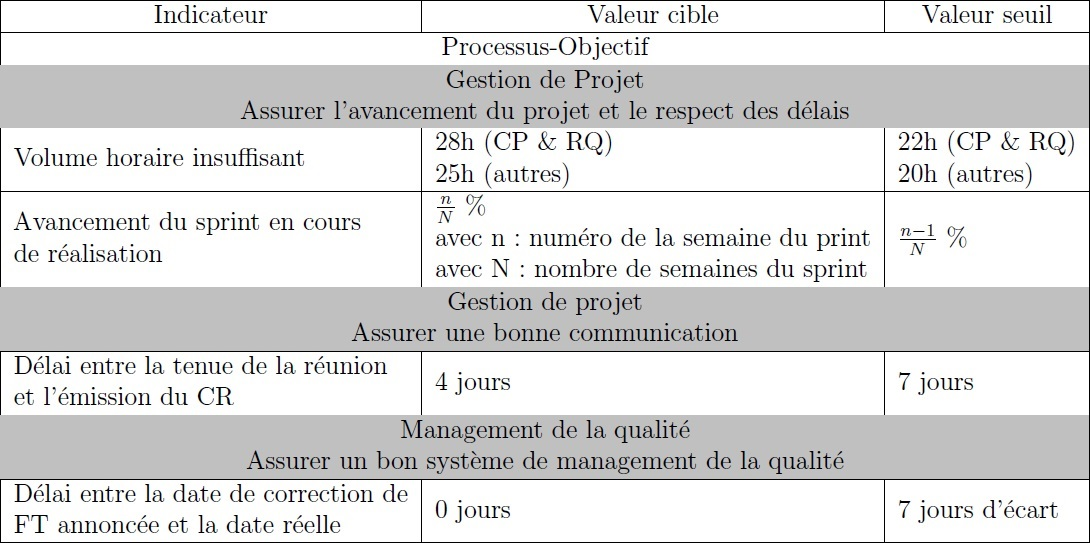
\includegraphics[width=13cm]{./images/Indicateurs_hebdomadaires.jpg}
\end{figure}

\subsubsection*{Indicateurs ponctuels}
\label{Indicateurs ponctuels}
\paragraph*{} Les indicateurs ponctuels permettent de décrire les résultats d’événements ponctuels tels que les audits, les questionnaires de satisfaction, etc.

\paragraph*{} Un tableau récapitulant les indicateurs ponctuels mis en place est disponible dans le tableau
6.2. Pour les indicateurs faisant référence à des délais, le comptage exclut les vacances scolaires.
\begin{figure}[h]
   \center
   \caption{\label{Tableau 6.2} Indicateurs ponctuels}
   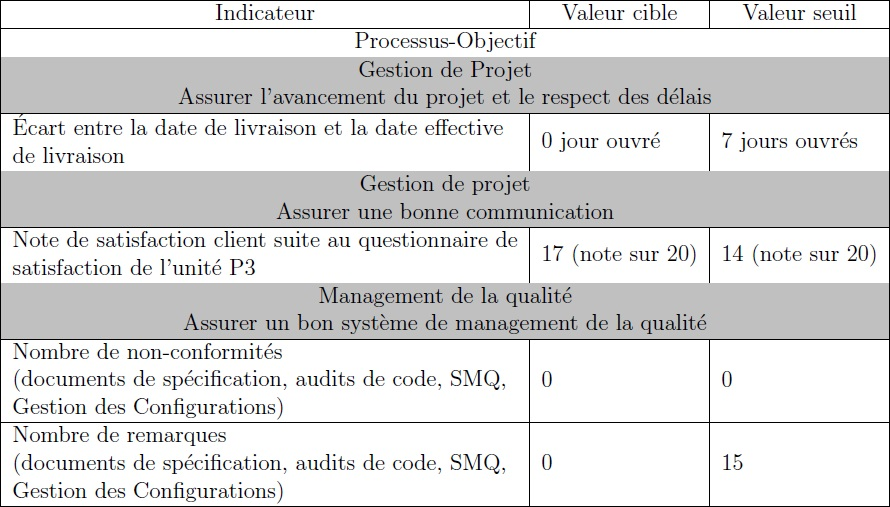
\includegraphics[width=13cm]{./images/Indicateurs_ponctuels.jpg}
\end{figure}

\subsubsection*{Tableau de bord}
\label{Tableau de bord}

\paragraph*{} Le \TB{} est un outil de suivi qui permet à l'équipe \nomEquipe{} de suivre visuellement l'évolution de la qualité grâce à la représentation des différents états des indicateurs
hebdomadaires.

\paragraph*{} Le \RQ{} sera en charge de la mise à jour de ce document, à raison d'une
fois par semaine. Chaque \TB{} sera imprimé, attaché dans la salle PIC, archivé
numériquement dans le \DSQ{} et en version papier dans l'armoire de la salle.

\section{Suivi de la qualité}
\label{Suivi de la qualite}
\subsection{Surveillance de la qualité du code}
\label{Surveillance de la qualite du code}
\paragraph*{} La surveillance de la qualité du code sera exécutée tout au long de la phase de codage du
PIC par le \RD , notamment grâce à des outils de vérification de règles de codage.

\paragraph*{} Une vérification de code aura lieu toutes les deux semaines. Elle sera menée par le \RD . En cas de besoin, ce dernier peut déléguer cette tâche à un autre membre
du PIC.

\paragraph*{} Les rapports consécutifs à ces vérifications seront archivés une fois les tests exécutés. De plus, un audit sera programmé au besoin par l'unité P3.

\subsection{\FT}
\paragraph*{} Le système de traitement des Faits Techniques (\FTCourt) assure un bon suivi de la qualité dans
le PIC.

\paragraph*{} L'enregistrement d'un \FT{} sur \lintranet{} permet de faire constater qu'un écart ou
qu'une insatisfaction a été relevé. Il témoigne donc de l'enregistrement et de la prise en compte
du problème par l'équipe PIC.

\paragraph*{} Un \FTCourt{} est corrigé par un \OC{} (\OCCourt), lui aussi enregistré grâce à l'outil
\lintranet .

\subsubsection*{\FT}
\paragraph*{} Un \FT{} peut découler d'une remarque venant d'une source qui peut être :

\begin{itemize}
	\item le client (remarques, points à modifier...) ;
	\item l'équipe PIC (problèmes internes, de planning, ...) ;
	\item un audit PIC ;
	\item une inspection.
\end{itemize}

\paragraph*{} Un \FTCourt{} a une gravité qui peut être :
\begin{itemize}
\item mineure : n'implique aucun retard dans le déroulement du projet ;
\item gênante : peut retarder la tâche mais pas le projet ;
\item très gênante : risque fortement d'entraîner un retard dans le projet ;
\item bloquante : bloque le déroulement.
\end{itemize}

\paragraph*{} De même, un \FTCourt est caractérisé par un type qui peut être :
\begin{itemize}
\item anomalie ;
\item remarque ;
\item actualisation ;
\item demande d'évolution ;
\item demande de correction.
\end{itemize}

\paragraph*{} Un \FTCourt{} permet de faire état d'un écart. Si plusieurs écarts sont constatés dans un même
document, ceux-ci peuvent éventuellement être regroupés au sein d'un même \FTCourt . Ce \FTCourt{} sera
clôturé après clôture de l'\OCCourt{} correspondant. Chaque \OCCourt{} devra être vérifié.
\paragraph*{} Une action demandée par un \OCCourt{} peut être :
\begin{itemize}
\item préventive ;
\item corrective ;
\item curative.
\end{itemize}

\paragraph*{} On privilégiera la mise en place d'actions préventives dans le cas d'identification préalable
d'un risque et d'actions correctives dans le cas d'identification d'un problème avéré.


\subsubsection*{\CTFT (\CTFTCourt)}
\paragraph*{} Les \CTFTCourt{} auront lieu à intervalles réguliers et seront adaptables en fonction du nombre de \FTCourt{} à
traiter.

\paragraph*{} Une \CTFTCourt{} permet d'étudier les différentes \FTCourt{} en cours et est composée des personnes
suivantes :
\begin{itemize}
\item les auteurs des \FFTCourt{} dans la mesure du possible ;
\item les responsables de corrections si besoin ;
\item les vérificateurs ;
\item la personne en charge de la clôture des \OCCourt .
\end{itemize}

\subsubsection*{Cycle d'un \FTCourt}
Le cycle d'un \FTCourt{} est présenté dans la figure 6.3.

\begin{figure}[h]
   \center
   \caption{\label{Figure 6.1} Cycle d'un \FT}
   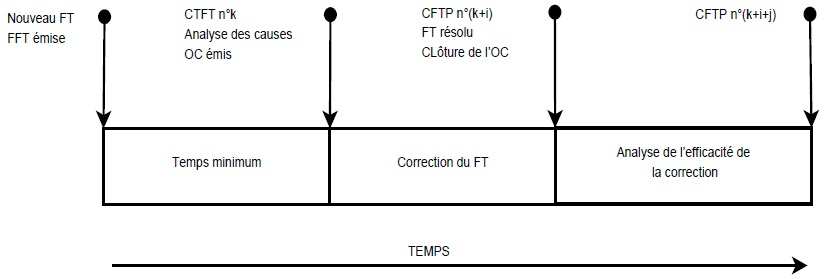
\includegraphics[width=13cm]{./images/cycle_Dun_FT.jpg}
\end{figure}

\subsubsection*{\FTCourt relatifs aux documents soumis à l’approbation}
\paragraph*{} Les demandes de modification(s)/évolution(s)/correction(s) de documents soumis à approbation ne feront pas l'objet d'émission de \FTCourt{} si les dites modification(s)/évolution(s)/correction(s) ne concernent que la forme du document (orthographe, mise en page...).

\subsection{Audits internes}
\paragraph*{} Conformément à la Norme ISO 9001:2015 , des audits internes (un durant le premier semestre et un durant le second) seront menés pour évaluer le management de la Qualité au sein du PIC et déterminer si le \SMQCourt{} est conforme :
\begin{itemize}
\item aux exigences de la Norme ISO 9001:2015 ;
\item au \SMQ{} de l'Unité P3 du département \ASI ;
\item aux dispositions prises par la direction du PIC (engagements, \PQCourt , \PGCCourt).
\end{itemize}
\paragraph*{} La mise en place d'un tel audit consiste à vérifier que les dernières versions des documents
Qualité du PIC sont cohérentes et à jour ainsi qu'à effectuer une surveillance des configurations.
Toute remarque ou non-conformité fera l'objet d'une \FFTCourt .

\paragraph*{} Pour chaque audit, un enregistrement de l'audit et de ses résultats sera établi et conservé
puis une vérification sera faite dans le but de contrôler que la correction des éventuelles non-conformités a été faite dans le temps imparti.

 
\chapter{Vérification et validation}
\label{verification_et_validation}
Chaque document produit par le PIC doit faire l'objet d'une vérification, d'une validation
et d'une approbation avant diffusion. Ce cycle est présent et décrit dans le \PGC (\PGCCourt). Il est cependant rappelé ici de façon à faciliter la recherche d'informations concernant ce cycle.

\section{Vérification}

\subsubsection*{A faire avant de commencer la vérification}
Avant toute chose, il est nécessaire de vérifier sur la plate-forme installée sur le serveur
(\lintranet) que le rédacteur a bien signalé que la rédaction du document est terminée.

\subsubsection*{A faire pour la vérification}
Le vérificateur doit vérifier les points suivants :
\begin{itemize}
\item vérification orthographique du document ;
\item vérification de la mise en page ;
\item vérification du suivi du document.
\end{itemize}
Des commandes LATEX peuvent être mises en place par exemple dans le cas où le rédacteur
n'est pas sûr sur un certain point. Ces commandes peuvent insérer des caractères dans le texte.
Le vérificateur devra vérifier qu'il n'y a plus d'insertion de ce type dans le document.

\subsubsection*{A faire après avoir effectué la vérification}

Après avoir vérifié un document, la personne en charge de cette tâche devra :
\begin{itemize}
\item le signaler sur \lintranet ;
\item signer le document papier si nécessaire ;
\item modifier le document numérique pour indiquer la date et indiquer qu'il a appliqué son
visa.
\end{itemize}

Le visa dans le document numérique peut être matérialisé de trois façons différentes :
\begin{itemize}
\item \lintranet : le visa est matérialisé seulement sur \lintranet par une case cochée.
\item Courriel : le visa a été matérialisé par courriel.
\item Signé : le visa a été matérialisé sur le document papier par une signature.
\end{itemize}

\subsection{Validation}

\subsubsection*{A faire avant de commencer la validation}
Le validateur doit vérifier que le vérificateur a bien indiqué sur \lintranet et sur le document que le document en question est vérifié.

\subsubsection*{A faire pour la validation}
Le validateur doit valider les points suivants :
\begin{itemize}
\item la pertinence du document ;
\item la complétude du contenu par rapport aux objectifs fixés.
\end{itemize}

\subsubsection*{A faire après avoir effectué la validation}
Après avoir validé un document, la personne en charge de cette tâche devra :
\begin{itemize}
\item le signaler sur \lintranet ;
\item signer le document papier si nécessaire ;
\item modifier le document numérique pour indiquer la date et indiquer qu'il a appliqué son
visa.
\end{itemize}

Le visa dans le document numérique peut être matérialisé de trois façons différentes :
\begin{itemize}
\item \lintranet : le visa est matérialisé seulement sur \lintranet par une case cochée.
\item Courriel : le visa a été matérialisé par courriel.
\item Signé : le visa a été matérialisé sur le document papier par une signature.
\end{itemize}


\subsection{Approbation}

Pour les documents qui ont une portée extérieure au PIC, une approbation sera nécessaire par la personne concernée extérieure au PIC. Le document une fois approuvé devient un enregistrement.

\subsubsection*{Approbation par les tuteurs}
Après chaque réunion avec un des tuteurs, un compte rendu ayant parcouru le cycle de
vérification et validation doit être approuvé.


\subsubsection*{Approbation par les tuteurs}
En ce qui concerne les documents approuvables par le client, si aucune remarque n'est effectuée
par le client sur le relevé de conclusions de réunions sous sept jours après l'envoi de ce dernier,
le compte-rendu est considéré comme approuvé.

\subsection{Diffusion}
Une fois approuvé (si le document nécessite une approbation), le document peut être diffusé.
Pour les documents sans approbation, c'est le rédacteur qui le diffuse. Pour le reste, c'est au
Chef PIC de s'en charger.

\section{Vérification et validation de lots}
Pour certaines livraisons, il se peut que le lot soit un ensemble de documents. Dans ce cas,
le vérificateur doit vérifier que tous les documents sont présents.
\\
Ce vérificateur devra rédiger un \PVVV (\PVVVCourt).

\chapter{Procédures et description de mesure d'analyse, Amélioration SMQ}
\label{mesure_analyse_amelioration_SMQ}
\section{Procédures et déscription de mesure d'analyse et d'amélioration du SMQ}\label{qualite}

Concernant cette partie ainsi que la description de la procédure de traitement des faits techniques, se reporter à la partie "Procédures et description du management de la qualité" et "Procédures et description de la vérification, surveillance et validation des documents"


\chapter{Management des ressources du projet}
\label{ressources}
\section{Organisation} \label{Organisation}

L'organigramme visible en figure \ref{organigramme} ci-dessous présente les ressources humaines et leurs rôles principaux associés.

\begin{figure}[H]
   \centering
   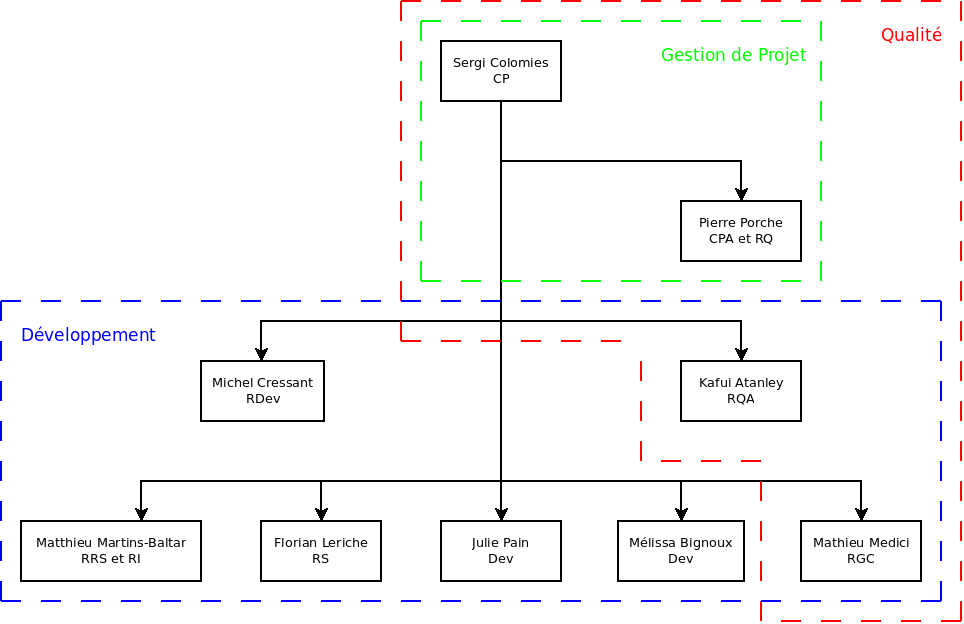
\includegraphics[width=15cm]{images/organigramme.png}
   \caption{\label{organigramme} Organigramme de \nomEquipe}
\end{figure}

\section{Compétences et formations} \label{CompetencesEtFormations}
\subsection{Rôles et compétences} \label{RolesEtCompetences}

\indent Chaque membre de l'équipe \nomEquipe{} est associé à un ou plusieurs rôles que l’on peut voir dans l’organigramme présenté ci-avant.\\

\indent Par défaut chaque membre possède le rôle de Développeur. On lui ajoute ensuite un rôle spécifique si nécessaire. Il pourra se voir attribuer le rôle de Pilote de Risque si celui-ci prend en charge la gestion d’un risque particulier.\\ 

\indent Le rôle de Responsable des Indicateurs sera également ajouté au Responsable Qualité, qui sera chargé de la mise à jour des indicateurs et du tableau de bord. \\

\indent Chaque attribution de rôle est justifiée par des compétences spécifiques que le titulaire doit posséder. C’est pourquoi les fiches de rôles spécifient les compétences requises pour effectuer une tâche. Ces fiches sont disponibles en annexe \ref{annexeFRo}. \\

\indent Ces Fiches de compétences, figurant dans le Dossier de Suivi de la Qualité, permettent de suivre le plan de formation de chaque membre de l’équipe PIC. Le formalisme d’une telle Fiche de compétences est disponible en annexe \ref{annexeFC}.\\

\indent Certaines personnes ont également des rôles plus particuliers détaillés dans la table \ref{repartRoles}. Chacun de ces rôles est défini dans une fiche de rôle disponible en annexe \ref{annexeFRo}.\\

\begin{table}[H]
\begin{tabular}[h]{|p{0.25\textwidth}|p{0.7\textwidth}|}
	\hline
	\rowcolor[gray]{0.85}
	Membre équipe PIC & Rôle(s) dans le projet \\\hline
	\Sergi &  \CP \\\hline
	\Pierre & \CPA, \RQ, \RI \\\hline
	\Kafui & \RQA, \D \\\hline
	\Mathieu & \RGC, \D \\\hline
	\Michel & \RD \\\hline
	\Matthieu & \RRS, \D \\\hline
	\Florian & \D \\\hline	
	\Julie & \D \\\hline
	\Melissa & \D \\\hline
\end{tabular}
\caption{\label{repartRoles} Répartition des rôles}
\end{table}

\subsection{Formations} \label{formation}

Si l'un des titulaires d'une tâche n'a pas les compétences requises pour la réaliser, il doit suivre une formation. Cette formation peut être organisée par un professeur, un autre membre de l'équipe PIC ou une personne externe. Si aucune de ces solutions n'est envisageable, le titulaire pourra s'autoformer.\\

Le temps nécessaire à une formation fait partie du planning du PIC et il apparaitra comme une tâche dans le planning. \\

Dans le cas où tous les membres du PIC devront s'autoformer à une technologie spécifique, deux membres du PIC devront réaliser un \QCM.

Un des deux \QCMCourt{} sera choisi pour que tous les membres du PIC soient évalués sauf le rédacteur de ce même \QCMCourt{} qui passera le second \QCMCourt.

Pour qu'une personne valide la formation, il faut que le \QCMCourt{} soit réussi à 66\% minimum. En cas d'échec à une évaluation, le membre devra se former de nouveau et repasser un \QCMCourt{} réalisé par un membre du PIC ayant obtenu cette compétence.

\section{Présence des membres}
\label{Présence des membres}

\subsection{Le temps de travail}
\label{temps_de_travail}
Selon le contrat d'étude, chaque membre de l'équipe doit faire un total de 24 heures de travail par semaine comprenant cinq jours ouvrés sur le PIC. Le Chef PIC et le Responsable Qualité possédant deux crédits de plus chacun, ils devront effectuer 27 heures par semaine comprenant cinq jours ouvrés. Si un ou quelques jours parmi ces cinq jours ouvrés sont fériés ou banalisés, on retire du volume horaire attendu les heures réservées à la réalisation du PIC sur ces jours fériés ou banalisés.

\subsection{En salle PIC}
\label{en_salle_pic}
Pour chaque membre, il est obligatoire de travailler minimum 18 heures en salle PIC par semaine comprenant cinq jours ouvrés. Pour le Chef PIC et le Responsable Qualité ce temps est de 20 heures par semaine comprenant cinq jours ouvrés. Si un ou quelques jours parmi ces cinq jours ouvrés sont fériés ou banalisés, on retire du volume horaire attendu les heures réservées à la réalisation du PIC sur ces jours fériés ou banalisés.\\

Un planning détaillé recensant les heures en salle de chaque membre sera créé et affiché.
Ce planning sera un moyen pour que le Chef PIC estime les ressources humaines disponibles à n'importe quel moment de la semaine.

\section{Locaux de réalisation du projet}
\label{Locaux de réalisation du projet}
\indent L'INSA, et plus précisément le département \ASI{}, met à disposition de chaque une salle de travail située dans le bâtiment Bougainville. Chaque équipe PIC bénificie de cette salle pour toute la durée du projet.
Concernant notre équipe, \nomEquipe, la salle qui nous a été attribué est ARC04.

\section{Inventaire du matériel mis à disposition}
\label{Inventaire du matériel mis à disposition}
Notre salle PIC a été fournie avec du matériel informatique dont l'inventaire est le suivant : \ref{annexeInventaire}.

\section{Inventaire des ressources informatiques}
\label{Inventaire des ressources informatiques}
Les ressources mises à disposition par le département \ASI{} pour l'équipe Unipik sont :

\begin{itemize}
	\item Un dépôt \git{} sur la plate-forme MonProjet de l'INSA Rouen;
	\item Un logiciel de gestion de projet PGPic.\\
\end{itemize}

Cependant il est possible que d'autres logiciels soient utilisés par l'équipe PIC tout au long du projet à condition que ceux-ci soient libres de droit d'utilisation.

\section{Matériel à acheter}
\label{Matériel à acheter}
\indent Aucun budget n'a été défini concernant le projet, l'application doit etre le plus proche possible de la gratuité (utilisation de logiciels et technologies issus du monde libre). \\
\indent Le secrétariat du département tient à jour un tableur où sont stockés les suivis de budget de toutes les équipes PIC.

\section{Eventuelle licence informatique à commander}
\label{Eventuelle licence informatique à commander}
\indent Pour le moment aucun achat de licence n'est nécessaire au projet.

\section{Matériel et/ou logiciel fournis par le client}
\label{Matériel et/ou logiciel fournis par le client}
\indent Pour le moment aucun prêt de matériel et/ou logiciel n'a été fait par le client.
\indent Dans le cas où des données seraient fournies à l’équipe PIC par le client, il faut faire un Procès-Verbal de réception à la récupération des données. A la fin du PIC, un Procès-Verbal de destruction des données doit être fait, pour certifier que les données ainsi que toutes les copies ont bien été détruites.

\section{Description des procédures relatives à l'écoute client}
\label{DescrProceduresRelativesALecouteClient}
\indent La communication avec le client devra s'effectuer à travers les documents de spécification interne et externe (\DSECourt , \DSICourt) (cf machin). Dans ces documents, les attentes du client seront prises en compte afin le satisfaire au maximum. Des réunions régulières devront également être réalisées ainsi qu'un \CRC{} après chaque réunion. Celui-ci devra être validé par le client afin d'éviter les incompréhensions entre les deux partis. \\
Les procédures à effectuer lors d'une réclamation ou une remarque du client devront être différenciées et sont décrites dans les parties suivantes.
   
\subsection{Remarques du client}
\label{RqClient}
A chaque remarque faite du client, une \FFT{} devra être réalisée (voir Annexe D \ref{fft}).

\subsection{Réclamations du client}
\label{ReclamClient}
A chaque réclamation du client, une \FFT{} (voir Annexe D \ref{fft})devra également être réalisée et un e-mail devra être envoyé au client. 


 
\begin{appendix}
\part*{Annexes}
\addcontentsline{toc}{part}{Annexes}

\chapter{Check-list de Vérification}
\label{annexeCheckList}
% version 1.00	Auteur Mélissa Bignoux

\begin{table}[H]
\centering
 \begin{tabular}{|l | c|}
 \hline
 \cellcolor{gray!40} Vérifier les pages de service & $\square$ \\
 \hline
  ~~Vérifier les dates du document & $\square$ \\
  ~~Vérifier les dates de suivi de diffusion & $\square$ \\
  ~~Vérifier la correction des FFT correspondantes & $\square$ \\
  ~~Vérifier la présence d'un tableau de définitions & $\square$ \\
  ~~Vérifier la présence d'un tableau d'abréviations & $\square$ \\
  ~~Vérifier le mode de diffusion & $\square$ \\
  \hline
 \cellcolor{gray!40} Respect de la langue française & $\square$ \\
 \hline
  ~~Fautes de français & $\square$ \\
  ~~Vérification de la ponctuation & $\square$ \\
  ~~Concordance du formalisme des listes & $\square$ \\
 \hline
 \cellcolor{gray!40} Structure et mise en page du document & $\square$ \\
 \hline
  ~~Vérification de la présence de la légende pour les figures & $\square$ \\
  ~~Vérification de la présence de la légende pour les tableaux & $\square$ \\
  ~~Cohérence dans la numérotation des parties du document & $\square$ \\
  ~~Cohérence des références & $\square$ \\
  ~~Vérifier la présence d'une liste des figures et d'une liste des tableaux & $\square$ \\
  \hline
  \cellcolor{gray!40} Vérifier l'adéquation des fichiers avec le PGC  & $\square$ \\
  \hline
 \end{tabular}
\end{table}


\chapter{Fiche de Risque}
\label{annexeFRi}
\section*{Informations générales}
 
\begin{table}[H]
\centering
	\begin{tabularx}{16.8cm}{|X|X|}
	\hline
	\rowcolor{gray!40} Numéro du risque & Type du risque \\
	\hline
	 &  \\
	\hline
	\end{tabularx}
\end{table}

\begin{table}[H]
\centering
	\begin{tabularx}{16.8cm}{|X|X|X|}
	\hline
	\rowcolor{gray!40} Date & Visa du \RQ & Visa du \CP \\
	\hline
	  & & \\
	\hline
	\end{tabularx}
\end{table}

\begin{table}[H]
\centering
	\begin{tabularx}{16.8cm}{|X|X|X|X|}
	\hline
	\rowcolor{gray!40} Pilote & Activité WBS & Compte WBS & Phase d'apparition \\
	\hline
	  & & &\\
	\hline
	\end{tabularx}
\end{table}

\section*{Description du risque}

\subsection*{Résumé}
	Indiquer ici un résumé du risque
	
\subsection*{Analyse des causes}
	Inclure un graphique issu de la méthode des n pourquoi afin d'identifier les différentes causes.

\subsection*{Criticité}

\begin{table}[H]
\centering
	\begin{tabularx}{16.8cm}{|>{\columncolor{gray!40}}X|X|}
	\hline
	Gravité & \\
	\hline
	Probabilité & \\
	\hline
	Criticité & \\
	\hline
	\end{tabularx}
\end{table}

\section*{Actions}
\subsection*{Actions préventives}

\begin{table}[H]
\centering
	\begin{tabularx}{16.8cm}{|X|X|}
	\hline
	\rowcolor{gray!40} Numéro de cause & Actions préventives \\
	\hline
	  & \\
	\hline
	\end{tabularx}
\end{table}

\subsection*{Plan de contournement}
Seront listés ici les différents plans de contournements permettant de contourner le risque

\chapter{Fiche d'opportunité}
\label{annexeFO}
\section*{Informations générales}
 
\begin{table}[H]
\centering
	\begin{tabularx}{16.8cm}{|X|X|}
	\hline
	\rowcolor{gray!40} Numéro de l'opportunité & Type de l'opportunité \\
	\hline
	 &  \\
	\hline
	\end{tabularx}
\end{table}

\begin{table}[H]
\centering
	\begin{tabularx}{16.8cm}{|X|X|X|}
	\hline
	\rowcolor{gray!40} Date & Visa du \RQ & Visa du \CP \\
	\hline
	  & & \\
	\hline
	\end{tabularx}
\end{table}

\begin{table}[H]
\centering
	\begin{tabularx}{16.8cm}{|X|X|X|X|}
	\hline
	\rowcolor{gray!40} Pilote & Activité WBS & Compte WBS & Phase d'apparition \\
	\hline
	  & & &\\
	\hline
	\end{tabularx}
\end{table}

\section*{Description de l'opportunité}

\subsection*{Résumé}
	Indiquer ici un résumé de l'opportunité.
	
\subsection*{Analyse des causes}
	Inclure ici un graphique issu de la méthode des n pourquoi afin d'identifier les différentes causes.

\subsection*{Criticité}

\begin{table}[H]
\centering
	\begin{tabularx}{16.8cm}{|>{\columncolor{gray!40}}X|X|}
	\hline
	Bénéfice & \\
	\hline
	Probabilité & \\
	\hline
	Criticité & \\
	\hline
	\end{tabularx}
\end{table}

\section*{Actions}
\subsection*{Actions proactives}

\begin{table}[H]
\centering
	\begin{tabularx}{16.8cm}{|X|X|}
	\hline
	\rowcolor{gray!40} Numéro de cause & Actions proactives \\
	\hline
	  & \\
	\hline
	\end{tabularx}
\end{table}


\chapter{Portefeuille de Risques et d'Opportunités}
\embedPDF{../PRO/pdf/PRO_Q_Unipik_V1.00.pdf}

\chapter{Fiche de Fait Technique}
\label{annexeFFT}
% version 1.00	Auteur Pierre Porche

\section*{Identification du \FTCourt}
\label{fft}
\begin{table}[H]
\centering
	\begin{tabularx}{16.8cm}{|>{\columncolor{gray!40}}l|X|}
	\hline
	Numéro de référence & \\
	\hline
	Identification du document (contenant le code \PICCourt{}) & \\
	\hline
	Date de création & \\
	\hline
	Type de \FTCourt* & \\
	\hline
	Prénom et Nom de l'auteur & \\
	\hline
	Source du \FTCourt** & \\
	\hline
	\end{tabularx}
\end{table}
\noindent \small * Anomalie, Remarque, Non-conformité, Actualisation, Demande d'évolution ou Demande de correction. \\
\small ** Audit \PICCourt{}, Inspection, Réclamation client ou interne.

\section*{Documents en référence}

\begin{table}[H]
\centering
	\begin{tabularx}{16.8cm}{|>{\columncolor{gray!40}}l|X|}
	\hline
	Référence et version de l'objet du \FTCourt & \\
	\hline
	Référence de la \CTFTCourt & \\
	\hline
	Référence à l'\OC & \\
	\hline
	Description & \\
	\hline
	Gravité* & \\
	\hline
	\end{tabularx}
\end{table}
\noindent \small * Sans conséquence, grave ou très grave.

\section*{Analyse des causes}

Quelle est la cause du \FT ? (méthode des n pourquoi)
\begin{itemize}
	\item
	\item
	\item
\end{itemize}

\section*{Clôture de la \FFTCourt}

\begin{table}[H]
\centering
	\begin{tabularx}{16.8cm}{|>{\columncolor{gray!40}}l|X|}
	\hline
	Référence de la \CTFTCourt & \\
	\hline
	Prénom et Nom & \\
	\hline
	Date & \\
	\hline
	Signature & \\
	\hline
	\end{tabularx}
\end{table}

\section*{Analyse à froid}

\begin{table}[H]
\centering
	\begin{tabularx}{16.8cm}{|>{\columncolor{gray!40}}l|X|}
	\hline
	Date de l'analyse & \\
	\hline
	Prénom(s) et nom(s) & \\
	\hline
	Avis sur l'efficacité de la ou des correction(s) & \\
	\hline
	Observations si correction(s) non efficace(s) & \\
	\hline
	\end{tabularx}
\end{table}

\chapter{Fiche de Commission de Traitement des Faits Techniques}
\label{annexeFCTFT}
% version 1.00	Auteur Pierre Porche

\begin{table}[H]
\centering
	\begin{tabularx}{16.8cm}{|>{\columncolor{gray!40}}l|X|}
	\hline
	Date de réunion de la CTFT &  \\
	\hline
	\end{tabularx}
\end{table}


\begin{center}
	Membres de la CTFT
\end{center}
\begin{table}[H]
\centering
	\begin{tabularx}{16.8cm}{|X|X|X|X|}
	\hline
	
	\cellcolor{gray!40} NOM & 
	\cellcolor{gray!40} PRENOM & 
	\cellcolor{gray!40} FONCTION & 
	\cellcolor{gray!40} Signature \\
	
	\hline
	 & & & \\
	\hline
	& & & \\
	\hline
	
	\end{tabularx}
\end{table}



\begin{table}[H]
\centering
	\begin{tabularx}{16.8cm}{|X|X|X|}
	\hline
	
	 \cellcolor{gray!40} Numéro FFT analysée & 
	 \cellcolor{gray!40} Date d'émission du FT &
	 \cellcolor{gray!40} Date de clôture du FT \\
	
	\hline
	 & &  \\
	\hline
	& &  \\
	\hline
	
	\end{tabularx}
\end{table}


\begin{center}
	Analyse des FFT émises
\end{center}


\begin{table}[H]
\centering
	\begin{tabularx}{16.8cm}{|X|X|X|}
	\hline
	
	 \cellcolor{gray!40} Numéro de fiche d'Ordre de Correction & 
	 \cellcolor{gray!40} Numéro(s) du(des) FFT concernée(s) & 
	 \cellcolor{gray!40} Date limite de correction \\
	
	\hline
	 & &  \\
	\hline
	
	
	\end{tabularx}
\end{table}

\begin{center}
	Rédaction d'Ordre de Correction au regard de l'analyse des FT
\end{center}



\begin{table}[H]
\centering
	\begin{tabularx}{16.8cm}{|X|X|X|X|X|}
	\hline
	
	 \cellcolor{gray!40} Numéro FFT &
	 \cellcolor{gray!40} Numéro OC &
	 \cellcolor{gray!40} Le délai entre l'émission du FT et son OC ne dépasse pas 10j ouvrés (OUI/NON) &
	 \cellcolor{gray!40} Le délai entre l'émission de l'OC et sa prise en compte ne dépasse pas 2j ouvrés (OUI/NON) &
	 \cellcolor{gray!40} La délai entre la date d'émission du FT et sa clôture ne dépasse pas trois semaines (OUI/NON)  \\
	
	\hline
	 & & & & \\
	\hline
	 & & & & \\
	\hline
	 & & & & \\
	\hline
	
	
	\end{tabularx}
\end{table}

\begin{center}
	Respect des délais
\end{center}


\chapter{Fiche d'Ordre de Correction}
\label{annexeFOC}
% version 1.00	Auteur Pierre Porche

\section*{Identifiant}

\begin{table}[H]
\centering
	\begin{tabularx}{16.8cm}{|>{\columncolor{gray!40}}l|X|}
	\hline
	Numéro de référence & \\
	\hline
	Identification du document (contenant le code \PICCourt) & \\
	\hline
	Date de création & \\
	\hline
	Date limite de correction & \\
	\hline
	Auteur & \\
	\hline
	Correcteur & \\
	\hline
	Fonction du correcteur & \\
	\hline
	Vérificateur & \\
	\hline
	\end{tabularx}
\end{table}

\section*{FFT concernée(s)}

\begin{table}[H]
\centering
	\begin{tabularx}{16.8cm}{|X|X|X|}
	\hline
	\rowcolor{gray!40} \FFTCourt{} concernée(s) & Type d'action* & Description de la correction à apporter \\
	\hline
	 & & \\
	\hline
	\end{tabularx}
\end{table}
\noindent \small * Corrective ou Préventive

\section*{Articles ouverts à la correction}

\begin{table}[H]
\centering
	\begin{tabularx}{16.8cm}{|X|X|X|}
	\hline
	\rowcolor{gray!40} Nom de l'article & Référence & Version après correction \\
	\hline
	 & & \\
	\hline
	\end{tabularx}
\end{table}

\section*{Vérification}

\begin{table}[H]
\centering
	\begin{tabularx}{16.8cm}{|>{\columncolor{gray!40}}l|X|}
	\hline
	Prénom et Nom & \\
	\hline
	Date de la vérification & \\
	\hline
	Avis* & \\
	\hline
	Signature & \\
	\hline
	\end{tabularx}
\end{table}
\noindent \small * Satisfaisant ou Insatisfaisant

\section*{Clôture}

Un \OCCourt{} sur un document soumis à approbation ne peut être clôturé sans que celui-ci ait été réapprouvé au préalable.

\begin{table}[H]
\centering
	\begin{tabularx}{16.8cm}{|>{\columncolor{gray!40}}l|X|}
	\hline
	Prénom et Nom & \\
	\hline
	Date de la clôture & \\
	\hline
	Signature & \\
	\hline
	\end{tabularx}
\end{table}

\chapter{Fiches de Rôle}
\label{annexeFRo}
\section{\CP}
\subsection*{Introduction}

<<<<<<< HEAD
Le \CP{} doit garantir le bon déroulement du \PICCourt. Il possède des missions d’organisation et de validation du travail effectué par les membres de l’équipe. Il est également l’interlocuteur privilégié du tuteur pédagogique, du tuteur qualité et du client.
=======
Le \CP{} doit garantir le bon déroulement du \PICCourt. Il possède des missions d’organisation et de validation du travail effectué par les membres de l’équipe. Il est également l’interlocuteur privilégié du Tuteur Pédagogique, du Tuteur Qualité et du client.
>>>>>>> 0df4c754161dfe55442977f5cea6b2c3513bd81b

\subsection*{Tâches liées à sa fonction}

Une passation devra être mise en place entre les \CPs{} du premier et second semestre. Cette passation devra si possible être formalisée sous la forme d’une formation.

\subsection*{Tâches effectuées au démarrage du \PICCourt}

Le \CP{} devra se conformer aux exigences de la période de démarrage du \PICCourt :
\begin{itemize}
	\item Organiser l’équipe \PICCourt au premier semestre et de la fin du premier au second semestre en tenant compte des éventuels départs à l’étranger, redoublements, réorientations ou retours de mobilité académique. Ainsi qu’organiser la formation en début du second semestre du \PICCourt
<<<<<<< HEAD
	\item Créer le dépôt \git{} sur https://monprojet.insa-rouen.fr et des espaces publics et privés des membres de l’équipe \PICCourt
=======
	\item Créer le dépôt \git sur https://monprojet.insa-rouen.fr et des espaces publics et privés des membres de l’équipe \PICCourt
>>>>>>> 0df4c754161dfe55442977f5cea6b2c3513bd81b
	\item Rédiger ou faire rédiger, puis valider les \FC{} de son équipe et éventuellement attester certaines compétences d’ordre personnel.
	\item Établir l’organigramme des fonctions de son \PICCourt et les descriptifs de ces fonctions.
	\item Associer les ressources aux fonctions de son \PICCourt.
\end{itemize}

\subsection*{Tâches effectuées au cours du \PICCourt}

Le \CP{} devra remplir au cours du \PICCourt les missions suivantes :

\begin{itemize}
	\item Mettre à jour les \FC{} des membres du \PICCourt.
	\item Archiver de manière hebdomadaire l’ensemble des espaces privés des membres et les conserver sur clé USB jusqu’à la semaine suivante.
	\item Garantir les journaux de tests.
	\item Participer à la \CTFT (CTFT).
	\item Gérer le budget de fonctionnement du \PICCourt.
<<<<<<< HEAD
	\item Représenter les ressources globales du \PICCourt et le solde des ressources consommées par un \WBSCourt minimal, un OBS, un \RBSCourt{} ou un \FBSCourt.
=======
	\item Représenter les ressources globales du \PICCourt et le solde des ressources consommées par un \WBSCourt{} minimal, un OBS, un \RBSCourt{} ou un \FBSCourt.
>>>>>>> 0df4c754161dfe55442977f5cea6b2c3513bd81b
	\item Collecter les risques de tâches mis en lumière par les membres de l’équipe.
	\item Participer à la réunion de la conduite de projet ou suivi prévisionnel tenue au minimum une fois par semestre.
	\item Effectuer le débriefing à la revue de \PICCourt.
	\item Accorder les dérogations de possibilité de diffusion des non-conformités en accord avec le client.
\end{itemize}

Le \CP{} devra également remplir ou déléguer ces missions au \CPA :
\begin{itemize}
	\item Animer la réunion d’avancement hebdomadaire.
	\item Établir les diagrammes de Gantt pour le suivi des tâches passées, en cours et futures.
	\item Reprendre le planning de la semaine passée et le mettre à jour en fonction des retards estimés, des réunions exceptionnelles et des corrections possibles.
	\item Vérifier les fiches de suivi hebdomadaire des membres de l’équipe.
\end{itemize}

\subsection*{Tâches effectuées en fin de période du \PICCourt}

Le \CP{} devra en fin de période remplir les missions suivantes :
\begin{itemize}
	\item Livrer au secrétariat de la Direction du Département \ASICourt{} l’archivage de l’espace public des membres de l’équipe en fin de semestre.
	\item Garantir avec la Direction Qualité dans un \PVCourt{} la fin de la phase d’intégration.
\end{itemize}
\newpage

\section{\CPA}
\subsection*{Introduction}

<<<<<<< HEAD
Durant le premier semestre, le \CPA{} doit seconder le \CP{} et effectuer les tâches qu’il lui aura délégué. À la fin de ce semestre, dans la majorité des cas, il devra se préparer à assurer le rôle de \CP.
=======
Durant le premier semestre, le \CPA{} doit seconder le \CP{} et effectuer les tâches qu’il lui aura déléguées. À la fin de ce semestre, dans la majorité des cas, il devra se préparer à assurer le rôle de \CP.
>>>>>>> 0df4c754161dfe55442977f5cea6b2c3513bd81b

\subsection*{Tâches liées à sa fonction}

Le \CPA{} devra remplir les missions suivantes :
\begin{itemize}
	\item Établir avec le \CP{} le planning détaillé des activités à réaliser ;
	\item Réaliser avec le \CP{} le suivi du projet ;
	\item Remplacer le \CP{} si celui-ci est indisponible ;
<<<<<<< HEAD
	\item Préparer le semestre suivant, en collaboration avec le \CP, à la fin du premier semestre, s’il prend la fonction de \CP{} au second semestre.
=======
	\item Préparer le semestre suivant, en collaboration avec le \CP{}, à la fin du premier semestre, s’il prend la fonction de \CP{} au second semestre.
>>>>>>> 0df4c754161dfe55442977f5cea6b2c3513bd81b
\end{itemize}

\newpage
\section{\RQ}
\subsection*{Introduction}

Le \RQ{} est le garant de l’application de la politique qualité au sein du \PICCourt. Il peut être épaulé dans cette tâche par d’autres membres du \PICCourt.

\subsection*{Tâches liées à sa fonction}

Une passation devra être mise en place entre les \RQs{} du premier et second semestre. Cette passation devra si possible être formalisée sous la forme d’une formation.\\
Tout au long du projet, le \RQ{} devra veiller à la bonne adéquation entre les tâches liées à la réalisation des livrables et le référentiel qualité. Pour assurer le bon déroulement de cette veille qualité, il devra réaliser les tâches suivantes :

\subsubsection*{Tâches liées au \PQCourt}
\begin{itemize}
<<<<<<< HEAD
	\item Rédiger et organiser le suivi du \PQ (\PQCourt) en respectant les exigences du Référentiel Qualité et en particulier de la \DGQDEUXCourt.
	\item Assurer la bonne diffusion (c’est à dire, l’envoi après approbation) du \PQCourt{} aux membres de l’équipe \PICCourt.
	\item Vérifier le \PQCourt{} après l’exécution d’actions correctives (cette tâche peut être déléguée à un autre membre du \PICCourt par dérogation personnelle ou de la part du \CP).
=======
	\item Rédiger et organiser le suivi du \PQ{} (\PQCourt) en respectant les exigences du Référentiel Qualité et en particulier de la \DGQDEUXCourt.
	\item Assurer la bonne diffusion (c’est à dire, l’envoi après approbation) du \PQCourt{} aux membres de l’équipe \PICCourt.
	\item Vérifier le \PQCourt{} après l’exécution d’actions correctives (cette tâche peut être déléguée à un autre membre du \PICCourt{} par dérogation personnelle ou de la part du \CP).
>>>>>>> 0df4c754161dfe55442977f5cea6b2c3513bd81b
	\item Valider l’ensemble des procédures qualité rédigées au sein du \PICCourt.
	\item Fournir un accompagnement aux équipes de développement dans la démarche qualité.
	\item Réaliser des activités régulières de contrôle de l’ensemble du système qualité.
	\item Sensibiliser les membres de l’équipe \PICCourt{} à la norme \ISOCourt 9001:2015.
\end{itemize}

\subsubsection*{Tâches liées au \PGCCourt}

Cette partie peut être déléguée dès le début du \PICCourt{} à un autre membre du \PICCourt{}, possédant la compétence exigée, qui prendra alors la responsabilité de la gestion des configurations.

\begin{itemize}
	\item Rédiger et organiser le suivi du \PGCCourt{} en respectant les exigences du Référentiel Qualité et en particulier de la \DGQDEUXCourt.
<<<<<<< HEAD
	\item Vérifier le \PGCCourt après l’éxécution d’actions correctives (cette tâche peut être déléguée à un autre membre du \PICCourt par dérogation personnelle ou de la part du \CP).
=======
	\item Vérifier le \PGCCourt{} après l’exécution d’actions correctives (cette tâche peut être déléguée à un autre membre du \PICCourt{} par dérogation personnelle ou de la part du \CP).
>>>>>>> 0df4c754161dfe55442977f5cea6b2c3513bd81b
	\item Garantir l’application du \PGCCourt.
	\item S’assurer du bon déroulement de la gestion des modifications des différents documents.
\end{itemize}

\subsubsection*{Tâches liées à la gestion du référentiel}

\begin{itemize}
<<<<<<< HEAD
	\item Chaque semestre, les \RQs{} doivent se réunir et fournir au pilote de processus 2, une liste de cinq questions par responsable visant à évaluer la maîtrise de ce référentiel ;
=======
	\item Chaque semestre, les \RQs{} doivent se réunir et fournir au pilote de processus 2, une liste de 5 questions par responsable visant à évaluer la maîtrise de ce référentiel ;
>>>>>>> 0df4c754161dfe55442977f5cea6b2c3513bd81b
	\item Chaque semestre, les \RQs{} doivent se réunir pour se répartir et corriger les demandes d’amélioration présentes sur l’outil de suivi des référentiels ;
	\item Chaque semestre, à chaque incohérence et problème soulevé, les \RQs{} doivent ajouter des demandes d’amélioration à l’aide de l’outil de suivi des référentiels.
\end{itemize}

\newpage
\section{\RQA}
\subsection*{Introduction}

Durant le premier semestre, le \RQA{} doit seconder le \RQ{} et effectuer les tâches qu’il lui aura déléguées. À la fin de ce semestre, dans la majorité des cas, il devra se préparer à assurer le rôle de \RQ .

\subsection*{Tâches liées à sa fonction}

Le \RQA{} devra remplir les missions suivantes :
\begin{itemize}
	\item Tenir à jour les différents indicateurs mis en place pour le \PICCourt.
	\item Remplacer le \RQA{} si celui-ci est indisponible ;
	\item Seconder le \RQ{} dans la réalisation du \PQ, du \PGC{} ainsi que des autres documents liés au projet.
        \item Participer au développement des fonctionnalités nécessaires au projet. 
\end{itemize}

\newpage
\section{\RGC}
\subsection*{Introduction}

Au début du projet, le \RGC{} doit s'occuper de la rédaction du \PGCCourt{} qui sert à contrôler l’activité de gestion des configurations pendant toute la durée du \PICCourt. L’élaboration de ce document permet donc de fixer toutes les règles de la gestion des configurations. Ce dernier sera amené à évoluer tout au long du projet afin que cette gestion soit toujours adaptée au \PICCourt.

\subsection*{Tâches liées à sa fonction}

Le \RGC{} devra remplir les missions suivantes :
\begin{itemize}
	\item Mettre en place le gestionnaire de sources du \PICCourt.
	\item Rédiger le \PGC.
	\item Fixer les règles de la gestion des configurations.
        \item Clôturer les ordres de corrections après avoir vérifié que la procédure de correction/vérification avait bien été respectée.
        \item Se charger de l'effacement du dépôt des sources.
        \item S'assurer que les membres de l'équipe \PICCourt{} respectent le \PGCCourt.
\end{itemize}

\newpage
\section{\RRS}
\subsection*{Introduction}

Au début du projet, le \RRS{} doit s'occuper de la mise en place du réseau dans la salle \PICCourt afin que chaque membre ait accès à internet et puisse travailler dans de bonnes conditions. Il sera chargé de maintenir ce réseau fonctionnel tout au long du projet.

\subsection*{Tâches liées à sa fonction}

Le \RRS{} devra remplir les missions suivantes :
\begin{itemize}
	\item Mettre en place le réseau en salle \PICCourt.
	\item S'assurer du bon fonctionnement du réseau tout au long du \PICCourt.
	\item S'assurer du bon état de fonctionnement du serveur.
	\item Faire évoluer l'architecture du réseau en fonction des besoins utilisateurs.
	\item Participer à la gestion technique des équipements. Cela consiste à réceptionner les matériels informatiques et de télécommunications, les tester, les adapter, les insérer dans le réseau en fonctionnement et effectuer le suivi du parc de matériels.
\end{itemize}

\newpage
\section{\RD}
\subsection*{Introduction}

Tout au long du projet, le \RD{} doit s'occuper de la gestion de toutes les parties concernant le développement. Il aura donc sous sa charge un certain nombre de développeurs et va devoir s'assurer que les résultats issus du développement sont conformes au \DGQDEUXCourt.

\subsection*{Tâches liées à sa fonction}

Le \RD{} devra remplir les missions suivantes :
\begin{itemize}
	\item Définir avec le \CP{} les différentes phases de conception et de développement.
	\item Établir les phases de vérification et de validation du développement.
<<<<<<< HEAD
	\item Participer à la réalisation du \DSECourt, du \DSICourt{} et du \PTVCourt.
=======
	\item Participer à la réalisation du \DSECourt{}, du \DSICourt{} et du \PTVCourt.
>>>>>>> 0df4c754161dfe55442977f5cea6b2c3513bd81b
	\item S'assurer de la réussite des tests unitaires et d'intégration.
	\item S'assurer que les codes fournis fonctionneront également chez le client.
\end{itemize}	

\chapter{Fiche de Compétences}
\label{annexeFC}
\documentclass[11pt]{article}
\usepackage{draftcopy}
\usepackage[francais]{babel}
\usepackage[utf8]{inputenc}
\usepackage{tabularx}
\usepackage{graphicx}
\usepackage[table]{xcolor}
\usepackage{fancyhdr}
\usepackage{../../../ressources/Unipik/vocabulaire/vocabulaireUnipik}
\usepackage{longtable}


\begin{document}

\chead{\huge Fiche de compétence}

\begin{center}
\begin{table}[!hp]

	\begin{tabularx}{\linewidth}{|X|X|}
	\hline
	\rowcolor{gray!40} Élève ingénieur & Date et signature \\
	\hline
	\end{tabularx}
	\begin{tabularx}{\linewidth}{|X|X|}
	Nom : tonNom & Date : XX/XX/2016 \\ 
	Prénom : TonPrenom & \\
	Semestre : Semestre 8 & \\
	\hline
	\end{tabularx}
\end{table}
\end{center}

\section*{\large\FR}

\centering
	\begin{longtable}{|p{4cm}|p{4cm}|}
	\hline
	\rowcolor{gray!40} Référence \WBSCourt & Description du rôle \\
	\hline
	 1.1 & Manager la qualité \\
	\hline
	 1.2 & Conduire le Projet \\
	\hline
	 1.3 & Réaliser les produits \\
	 \hline
	\end{longtable}


\section*{\large\FC}

\centering
	\begin{longtable}{|p{3cm}|p{3cm}|p{3cm}|p{3cm}|}
	\hline
	\rowcolor{gray!40} Référence & Compétence & Justificatif & Niveau \\
	\hline
	 BD & Base de données & Examen & Faible \\
	\hline
	\end{longtable}

\centering
	\begin{longtable}{|p{12cm}|}
	\hline
	\rowcolor{gray!40} Compétences à acquérir par formation complémentaire \\
	\hline
	  \\
	\hline
	\end{longtable}

\section*{\large Suivi de formation}

\centering
	\begin{longtable}{|p{1.2cm}|p{1.2cm}|p{1.2cm}|p{1.2cm}|p{1.2cm}|p{1.2cm}|p{1.2cm}|p{1.2cm}|}
	\hline
	\rowcolor{gray!40} \tiny Date début & \tiny Date fin & \tiny Intitulé Formation & \tiny Nature Formation & \tiny Evaluateur & \tiny Avis & \tiny Signature & \tiny Évaluation à froid \\
	\hline
	 & & & & & & & \\
	\hline
	\end{longtable}

\end{document}

\chapter{Inventaire}
\label{annexeInventaire}
\begin{center}
\begin{longtable}{|p{10cm}|c|c|}
\hline \multicolumn{1}{|c|}{\textbf{Matériel}} & \multicolumn{1}{c|}{\textbf{Enregistré}} & \multicolumn{1}{c|}{\textbf{Nombre réel dans la salle}} \\ \hline 
\endfirsthead

\multicolumn{3}{c}%
{{\bfseries \tablename\ \thetable{} }} \\
\hline \multicolumn{1}{|c|}{\textbf{Matériel}} &
\multicolumn{1}{c|}{\textbf{Enregistré}} &
\multicolumn{1}{c|}{\textbf{Nombre Réel dans la salle}} \\ \hline 
\endhead

\hline \multicolumn{3}{|r|}{{Suite sur la prochaine page}} \\ \hline
\endfoot

\hline \hline
\endlastfoot
		\hline serveur/parefeu: asi-pic-121107-03  & 1 & 1 \\
		\hline pc: asi-pic-121107-10 & 1 & 1 \\
		\hline pc: asi-pic-121107-07 & 1 & 1 \\
		\hline pc: asi-pic-121107-21 & 1 & 1 \\
		\hline pc: asi-pic-121107-20 & 1 & 1 \\
		\hline pc: asi-pic-121107-09 & 1 & 1 \\
		\hline pc: asi-pic-121107-16 & 1 & 1 \\
		\hline pc: asi-pic-121107-14 & 1 & 1 \\
		\hline pc: asi-pic-121107-08 & 1 & 1 \\
		\hline Câble en Y pour double sorties DVI & 1 & 1 \\ 
		\hline HP LaserJet P2035 (VNC3438061)& 1 & 1 \\ 
		\hline Câble USB imprimante & 1 & 1 \\ 
		\hline Écran 24” Dell E248WFP CZ-0G274H-74263-93d-17es & 1 & 1 \\ 
		\hline Écran 24” Dell E248WFP CZ-0G274H-74263-93d-17fs & 1 & 1 \\ 
		\hline Écran 24” Dell G2410t CN-0W222K-74445-93N-698U & 1 & 1 \\ 
		\hline Écran 24” Dell ST2420 CN-09WTC7-74261-135-0G7U & 1 & 1 \\ 
		\hline Écran 24” Dell ST2420 CN-09WTC7-74261-135-0FNU & 1 & 1 \\ 
		\hline Écran 24” Dell 2405FPW HU-OM6754-46633-597-OC6S F  & 1 & 1 \\ 
		\hline Écran 24” Asus VH242 97LMTF064903 & 1 & 1 \\ 
		\hline Écran 24” Asus VH242 A3LMIZ083772 & 1 & 1 \\ 
		\hline Écran 24” Asus VW246 89LMQS027751 & 1 & 1 \\
		\hline Écran 24” Asus VW246 A3LMIZ083764 & 1 & 1 \\	
		\hline Écran 24” IIyama ProLite X2485WS1120023700458 & 1 & 1 \\ 
		\hline Écran 24” IIyama ProLite X2485WS1120023700768 & 1 & 1 \\
		\hline Écran 24” IIyama ProLite X2485WS1120023700853 & 1 & 1 \\
		\hline Écran 24” LG Flatron W2443T-PF 003MAWLCM353 & 1 & 1 \\
		\hline Claviers USB & 12 & 12 \\ 
		\hline Souris optique USB & 12 & 12 \\ 
		\hline Switch TP-Link TL-SG1016D & 1 & 1 \\ 
		\hline Câbles RJ45 standards & 14 & 15 \\ 
		\hline Câbles RJ45 jaune & 1 & 1 \\ 
		\hline Câbles RJ45 bleu & 3 & 3 \\ 
		\hline Câbles RJ45 vert & 2 & 3 \\ 
		\hline Câbles RJ45 rouge & 1 & 1 \\ 
		\hline Câbles VGA & 15 & 16 \\ 
		\hline Câbles DVI & 6 & 6 \\ 
		\hline Multiprises X6 & 4 & 4 \\ 
		\hline Multiprises X4 & 1 & 1 \\
                \hline 
\caption[Inventaire]{Inventaire} \label{grid_mlmmh} \\
\end{longtable}
\end{center}

	
\listoffigures
\addcontentsline{toc}{chapter}{Table des figures}
	 
\listoftables
\addcontentsline{toc}{chapter}{Liste des tableaux}
\end{appendix}
\pageQuatriemeCouverture

\end{document}
